% !TEX program = lualatex
% !TEX encoding = UTF-8
%
% Guía 85: Tridimenciónate
% Grado 9 - Meta 29
% Fe y Alegría Colombia
%
% Compilar con: lualatex guia_85.tex
%

\documentclass[12pt,a4paper]{article}

% ========== PAQUETES ==========
\usepackage[utf8]{inputenc}
\usepackage[spanish]{babel}
\usepackage{geometry}
\geometry{margin=2cm, top=1.5cm, bottom=1.5cm}

% Matemáticas
\usepackage{amsmath}
\usepackage{amssymb}
\usepackage{amsthm}

% Tablas y colores
\usepackage{xcolor}
\usepackage{array}
\usepackage{colortbl}
\usepackage{tabularx}
\usepackage{multirow}
\usepackage{array}
\usepackage{tcolorbox}
\tcbuselibrary{skins,breakable} % recomendado




% Cajas y entornos destacados
\usepackage{tcolorbox}
\tcbuselibrary{skins,breakable}
\tcbset{
    before skip=0.5em,
    after skip=0.5em,
    top=0.3cm,
    bottom=0.3cm,
    left=0.3cm,
    right=0.3cm
}

% Listas y enumeraciones
\usepackage{enumitem}

% Código verbatim
\usepackage{fancyvrb}

% Gráficos
\usepackage{graphicx}
\usepackage{pgfplots}
\usepgfplotslibrary{colormaps}
\usepackage{tikz}
\usepackage{tikz-3dplot}
\usepackage{wrapfig}
\usepackage{multicol}
\setlength{\columnsep}{18pt}
\setlength{\columnseprule}{0.4pt}
\pgfplotsset{compat=1.18}
\usetikzlibrary{shapes.geometric, calc, arrows.meta, 3d, babel}
\usepackage{float}
\usepackage{caption}
\tcbuselibrary{skins,breakable}

% Enlaces
\usepackage[hidelinks]{hyperref}

% ========== CONFIGURACIÓN DE COLORES ==========
\definecolor{azuloscuro}{RGB}{41,72,137}
\definecolor{rojoclaro}{RGB}{220,80,80}
\definecolor{verdeclaro}{RGB}{100,180,100}
\definecolor{fondogris}{RGB}{240,240,240}
\definecolor{fondorosa}{RGB}{255,230,240}
\definecolor{fondoverde}{RGB}{230,255,240}
\definecolor{fondoazul}{RGB}{230,240,255}

% ========== CONFIGURACIÓN DE ESPACIADO ==========
% Reducir espacio entre secciones
\setlength{\parskip}{0.3em}
\setlength{\parindent}{0pt}

% Reducir espacio antes y después de listas
\setlist{nosep, topsep=0.3em, partopsep=0pt, itemsep=0pt}

% Reducir espacios verticales adicionales
\setlength{\abovedisplayskip}{6pt}
\setlength{\belowdisplayskip}{6pt}
\setlength{\abovedisplayshortskip}{3pt}
\setlength{\belowdisplayshortskip}{3pt}

% Ajustar espacio entre títulos de sección
\usepackage{titlesec}
\titlespacing*{\section}{0pt}{0.5em}{0.3em}
\titlespacing*{\subsection}{0pt}{0.4em}{0.2em}
\titlespacing*{\subsubsection}{0pt}{0.3em}{0.2em}

% ========== COMANDOS PERSONALIZADOS ==========
\newcommand{\seccion}[1]{\section*{#1}\addcontentsline{toc}{section}{#1}}

% ========== TÍTULO DEL DOCUMENTO ==========
\title{\textbf{Guía 85: Tridimenciónate}}
\author{Fe y Alegría Colombia}
\date{}

% ========== INICIO DEL DOCUMENTO ==========
\begin{document}

% ========== PORTADA ==========
\begin{titlepage}
    \centering
    \vspace*{2cm}

    {\Huge\bfseries Guía 85\par}
    \vspace{0.5cm}
    {\Large Meta 29\par}
    \vspace{0.3cm}
    {\Large GRADO 9\par}
    \vspace{1cm}

    {\LARGE\bfseries GUÍA DEL ESTUDIANTE\par}
    \vspace{1cm}

    {\Huge\bfseries TRIDIMENCIÓNATE\par}
    \vspace{2cm}

    \vfill

    {\large Fe y Alegría Colombia\par}
    {\large Código: CH-FyA-0501\par}
\end{titlepage}

\newpage

% ========== CRÉDITOS ==========
\section*{Guías de Aprendizaje de Cualificar Matemáticas}
\subsection*{Fe y Alegría Colombia}

\textbf{Fe y Alegría Colombia}\\
\textbf{Víctor Murillo}\\
Director Nacional

\textbf{Desarrollo de contenidos pedagógicos y educativos}\\
Jaime Benjumea - Marcela Vega

\textbf{Autores de la guía 85}\\
Francy Paola González Castelblanco\\
Andrés Forero Cuervo

\textbf{Coordinación pedagógica}\\
Francy Paola González Castelblanco\\
Andrés Forero Cuervo\\
GRUPO LEMA \url{www.grupolema.org}

\textbf{Revisores}\\
Jaime Benjumea\\
Francy Paola González Castelblanco

\newpage

% ========== CONTENIDO PRINCIPAL ==========

\section*{GRADO 9 - META 29 - PENSAMIENTOS MÉTRICO - ESPACIAL}

\begin{tcolorbox}[colback=fondoazul, colframe=azuloscuro, title=\textbf{Guía 85} (Duración 13 h), breakable]
\textbf{ACTIVIDAD 1}
\begin{itemize}[nosep]
    \item Clasificación de sólidos
    \item Descomposición de sólidos
    \item Estimación de volumen
    \item Vértices, caras y aristas
\end{itemize}

\textbf{ACTIVIDAD 2}
\begin{itemize}[nosep]
    \item Área de superficie de sólidos
    \item Comparación entre volumen y área superficial de sólidos
\end{itemize}
\end{tcolorbox}

\subsection*{META DE APRENDIZAJE N. 29}

Argumento y razono al aplicar propiedades espaciales a proyectos como el diseño de estructuras en arquitectura, y la construcción de represas, para resolver problemas que aporten al bienestar común, donde debo aproximar la forma o volumen de objetos con sólidos conocidos, hallar su área superficial y volumen (pirámides, conos, esferas) y usar escalas. Ubico y describo figuras en el plano, las transformo y describo cómo cambia (o no) su forma y tamaño, y con ello hago patrones decorativos de baldosas. Comprendo y uso el teorema de Pitágoras y profundizo en criterios de semejanza de triángulos (teorema de Tales), para encontrar distancias geográficas y alturas. Así, uso lo que ya sé para resolver nuevos problemas geométricos de mi entorno.

\subsection*{PREGUNTAS ESENCIALES, GUÍA 85:}

\begin{itemize}[nosep]
    \item ¿Cuál es la diferencia entre calcular el volumen exacto de un sólido y estimar su volumen? En la vida real, ¿cuál de las dos es más frecuente?
    \item ¿Cómo me ayuda descomponer un sólido para calcular o estimar su volumen?
    \item ¿Cómo se relacionan y se diferencian los conceptos de volumen y área superficial de un sólido?
    \item ¿Hay alguna relación entre el número de caras, vértices y aristas de un poliedro? ¿Cómo puedo explorar esta pregunta?
\end{itemize}

\subsection*{EVIDENCIAS DE APRENDIZAJE, GUÍA 85:}

\begin{itemize}[nosep]
    \item Descompongo un sólido en otros sólidos básicos
    \item Razono para hallar el volumen de una pirámide
    \item Razono para hallar el volumen de un cono
    \item Razono para hallar el volumen de una esfera
    \item Identifico las caras de un sólido y su naturaleza (planas o no planas)
    \item Razono para hallar el área superficial de una pirámide
    \item Razono para hallar el área superficial de de un cono
    \item Razono para hallar el área superficial de una esfera
\end{itemize}

\vspace{4mm}

%\newpage

% ========== ACTIVIDAD 1 ==========
\section*{ACTIVIDAD 1: DESCOMPONGAMOS SÓLIDOS}

\textit{Aprendamos a clasificar sólidos según su forma, a aproximar objetos reales mediante sólidos y calcular su volumen y a comprender la relación entre puntos, aristas y caras de poliedros.}

\subsection*{A) Activando saberes previos}

% En el preámbulo

\begin{tcolorbox}[enhanced, breakable,
	colback=fondoazul, colframe=azuloscuro, title=\textbf{RECUERDA QUE...}, breakable]
	\begin{itemize}[nosep]
		\item Podemos clasificar sólidos así:
		\begin{itemize}[nosep]
			\item \textbf{POLIEDROS}: todas sus caras son planas. Ej: cubo, tetraedro, pirámide.
			\item \textbf{NO poliedros}: tienen al menos una cara curva. Ej: cilindro circular, esfera, cono.
		\end{itemize}
		
		\item Un prisma es un poliedro que tiene dos caras iguales paralelas.
		\item Un poliedro regular es uno donde todas las caras son polígonos regulares iguales.
		\item El volumen de un prisma o de un cilindro circular es el área de su base por su altura.
		
		\begin{itemize}[nosep]
			\item % --- Prisma (texto "rodeando" a la imagen con sidebyside) ---
			\begin{tcolorbox}[enhanced, frame hidden, boxrule=0pt, colback=fondoazul,
				sidebyside, sidebyside align=top seam, sidebyside gap=8pt,
				righthand width=0.15\textwidth]
				Para un prisma cuya base es un triángulo equilátero de lado $X$ y altura $H$,
				el volumen es $V=\frac{\sqrt{3}}{4}X^2H$. El prisma tiene dos bases paralelas
				congruentes y caras laterales rectangulares. El volumen se obtiene como área
				de la base por la altura $H$.
				\tcblower
				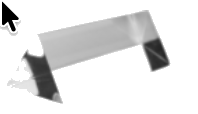
\includegraphics[width=\linewidth]{Figuras/fig2.png}
			\end{tcolorbox}
			
			\item % --- Cilindro ---
			\begin{tcolorbox}[enhanced, frame hidden, boxrule=0pt, colback=fondoazul,
				sidebyside, sidebyside align=top seam, sidebyside gap=8pt,
				righthand width=0.15\textwidth]
				Para un cilindro de radio $R$ y altura $H$, el volumen es
				$V=\pi R^2H$. Observa que depende del área del círculo base ($\pi R^2$) y
				de la altura del sólido.
				\tcblower
				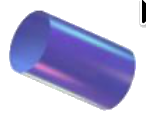
\includegraphics[width=\linewidth]{Figuras/fig3.png}
			\end{tcolorbox}
		\end{itemize}
		
		\item % --- Tetraedro ---
		\begin{tcolorbox}[enhanced, frame hidden, boxrule=0pt, colback=fondoazul,
			sidebyside, sidebyside align=top seam, sidebyside gap=8pt,
			righthand width=0.15\textwidth]
			Un tetraedro regular tiene 4 caras que son triángulos equiláteros de lado $X$.
			Se puede demostrar que su altura es $H=\tfrac{1}{3}\sqrt{6}\,X$ y su volumen
			$V=\tfrac{\sqrt{2}}{12}X^3$.
			\tcblower
			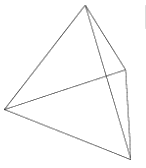
\includegraphics[width=\linewidth]{Figuras/fig4.png}
		\end{tcolorbox}
	\end{itemize}
\end{tcolorbox}


\begin{tcolorbox}[enhanced, breakable,
	colback=fondoverde, colframe=verdeclaro, title=\textbf{PRACTICA}]
	\textbf{i)} Completa esta tabla, marcando con \checkmark\ o X según el sólido tenga o no la propiedad dada.
	
	{\centering
		\small
		\renewcommand{\arraystretch}{1.4}
		\begin{tabular}{|>{\centering\arraybackslash}m{3cm}|
				>{\centering\arraybackslash}m{2cm}|
				>{\centering\arraybackslash}m{2cm}|
				>{\centering\arraybackslash}m{2cm}|
				>{\centering\arraybackslash}m{2cm}|
				>{\centering\arraybackslash}m{2cm}|}
			\hline
			\textbf{Sólido} & \textbf{Poliedro regular} & \textbf{Prisma} & \textbf{Poliedro} & \textbf{1 cara} & \textbf{Caras planas} \\
			\hline
			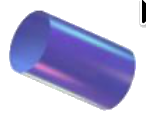
\includegraphics[width=1.5cm]{Figuras/fig3.png} &  &  &  &  &  \\ % Esfera
			\hline
			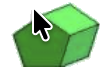
\includegraphics[width=1.5cm]{Figuras/fig7.png} &  &  &  &  &  \\ % Dodecaedro
			\hline
			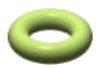
\includegraphics[width=1.5cm]{Figuras/fig8.png} &  &  &  &  &  \\ % Cilindro
			\hline
			
\includegraphics[width=1.5cm]{Figuras/fig9.png} &  &  &  &  &  \\ % Tetraedro
			\hline
			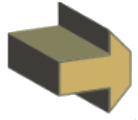
\includegraphics[width=1.5cm]{Figuras/fig10.png} &  &  &  &  &  \\ % Otro sólido
			\hline
		\end{tabular}\par}
	
	\vspace{5mm}
	
	% ==================== II ====================
	\begin{tcolorbox}[enhanced, frame hidden, boxrule=0pt, colback=fondoverde,
		sidebyside, sidebyside align=top seam, righthand width=0.09\textwidth,
		sidebyside gap=8pt]
		\textbf{ii)} Halla el volumen de un cilindro circular cuya base tiene un área de $12\pi$ unidades cuadradas, y cuyo radio de la base, $R$, es la cuarta parte de la altura, $H$.
		\tcblower
		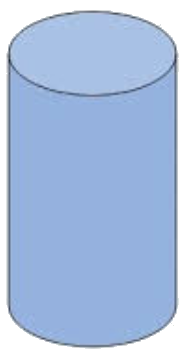
\includegraphics[width=\linewidth]{Figuras/fig5.png}
	\end{tcolorbox}
	
	\vspace{3mm}
	
	% ==================== III ====================
	\begin{tcolorbox}[enhanced, frame hidden, boxrule=0pt, colback=fondoverde,
		sidebyside, sidebyside align=top seam, righthand width=0.15\textwidth,
		sidebyside gap=8pt]
		\textbf{iii)} Considera un tetraedro regular en donde cada lado de cada triángulo equilátero mide 6 unidades.  
		Basado en esto, encuentra el volumen del tetraedro.
		\tcblower
		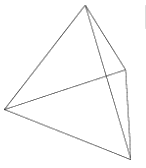
\includegraphics[width=\linewidth]{Figuras/fig4.png}
	\end{tcolorbox}
\end{tcolorbox}


\vspace{4mm}

%\newpage

\subsection*{B) Conceptos}

\subsubsection*{Exploración: Prototipando ando}

\begin{tcolorbox}[colback=fondoverde, colframe=verdeclaro]
Antes de comenzar discute en clase: ¿Haz hecho cerámica, carpintería, diseño gráfico en computadores u otro oficio de construcción de objetos? Describe tu experiencia.
\end{tcolorbox}

Una diseñadora gráfica hará objetos para una exposición arquitectónica. Diseñar un objeto implica:

\begin{itemize}[nosep]
    \item Hacer un prototipo del objeto, \textbf{DESCOMPONIÉNDOLO} en 1 o varios sólidos sencillos de fabricar. Estos sólidos se llaman ``módulos''.

    A veces aproximamos formas: por ejemplo, una naranja NO es es una esfera perfecta, pero es razonable pensar que sí lo es.

    \item Contar las ``puntas'', ``líneas de borde'' y ``lados'' de ciertos módulos, si es posible, para saber cuántas puntillas, silicona o pintura vamos a necesitar. Estos tres elementos los llamamos así:

    \textbf{Puntas = VÉRTICES ; Líneas de borde = ARISTAS ; Lados = CARAS}
\end{itemize}

\textbf{Sólidos básicos que usará la diseñadora:}

\begin{center}
	\small
	\renewcommand{\arraystretch}{1.25}
	\begin{tabular}{|p{4cm}|p{4cm}|p{4cm}|}
		\hline
		\textbf{Cilíndricos} & \textbf{Puntiagudos} & \textbf{Esféricos} \\
		\hline

		% --- Col 1: Prisma ---
		\textbf{Prisma}\par
		{\centering 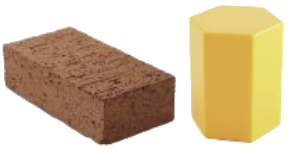
\includegraphics[width=3cm]{Figuras/fig13.png}\par}
		En particular, cubos, ortoedros (``Ladrillos'').\par
		Volumen: se multiplica el área de la base por la altura.
		&
		% --- Col 2: Pirámide ---
		\textbf{Pirámide}\par
		{\centering 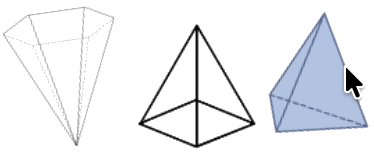
\includegraphics[width=3cm]{Figuras/fig15.png}\par}
		En particular, tetraedro, pirámide rectangular.\par
		Volumen: un tercio del volumen del prisma más pequeño que la contendría.
		&
		% --- Col 3: Esfera ---
		\textbf{Esfera y hemisferio} (``Pelotas'')\par
		{\centering 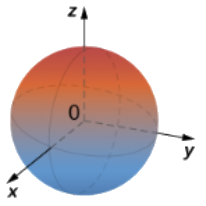
\includegraphics[width=3cm]{Figuras/fig17.png}\par}
		Volumen de una esfera de radio $R$:
		\[
		\frac{4}{3}\pi R^3
		\]
		\\
		\hline
			\end{tabular}
	\end{center}
	
	
		\begin{center}
		\small
		\renewcommand{\arraystretch}{1.25}
		\begin{tabular}{|p{4cm}|p{4cm}|p{4cm}|}
		\hline
		\textbf{Cilíndricos} & \textbf{Puntiagudos} & \textbf{Esféricos} \\
		\hline
		% --- Col 1: Cilindro ---
		\textbf{Cilindro circular}\par
		{\centering 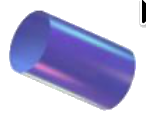
\includegraphics[width=3cm]{Figuras/fig3.png}\par}
		(Base circular)\par
		Volumen: se multiplica el área de la base por la altura.
		&
		% --- Col 2: Cono ---
		\textbf{Cono}\par
		{\centering 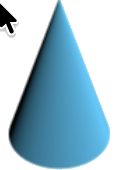
\includegraphics[width=1.7cm]{Figuras/fig16.png}\par}
		Volumen: un tercio del volumen del cilindro circular más pequeño que lo contendría.
		&
		% --- Col 3 vacío (como en tu tabla original) ---
		\\
		\hline
	\end{tabular}
\end{center}


\vspace{4mm}

%\newpage

\begin{multicols}{2}
	
	\subsubsection*{¡Manos a la obra!}

\textbf{i) Un sofá (casi) plano:}

\textbf{Descomposición:} Olvidando las patas para hacer más simple todo, podemos pensar en el sofá como un sólido compuesto por dos ortoedros (``ladrillos'') que están pegados.

Cada prisma tiene 8 puntas (Vértices), 12 bordes (Aristas) y 6 caras (en eso es igual a un dado): $(V, A, C) = (8, 12, 6)$

Para estimar el volumen del sofá, basta hallar el volumen de cada pieza y sumarlos.

Pero para hallar el área de superficie debemos sumar las áreas de cada prisma, y luego restar 2 veces el área de la cara donde ellas se pegan (ya que esta cara no es visible, así que no se pintaría en el sofá).

\begin{center}
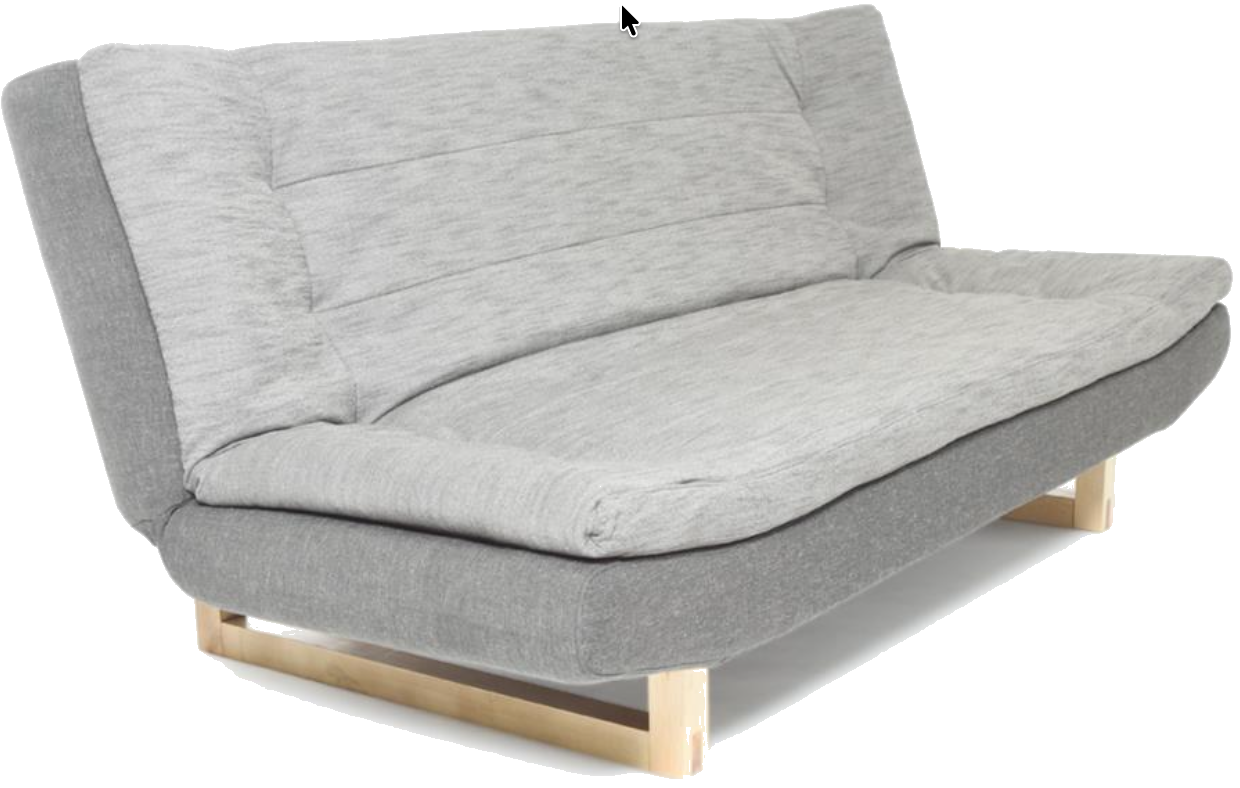
\includegraphics[width=0.8\columnwidth]{Figuras/fig18.png}
\end{center}

\textbf{Otra descomposición:} Al mirar al sofá de lado, vemos una cara poligonal en forma de L algo torcida:
Si ``replicamos'' (copiamos) este polígono a lo largo del ancho del sofá, obtenemos todo el sofá. Así, el sofá puede verse como un \textbf{PRISMA}, cuyas caras paralelas son los polígonos en forma de L.
Esto es, el sofá es un cilindro cuya base es un polígono en forma de L.

\begin{center}
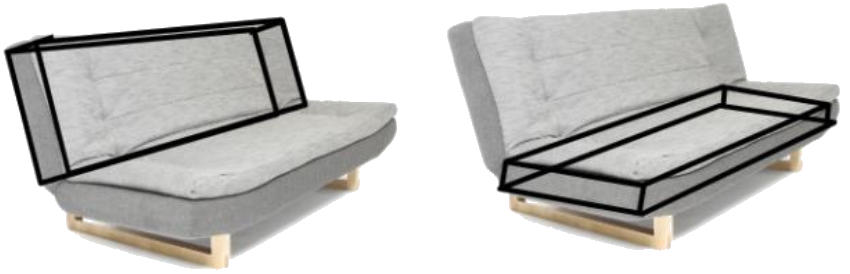
\includegraphics[width=0.9\columnwidth]{Figuras/fig19.png}
\end{center}

¡Dibújalo a partir de las L's!

\begin{center}
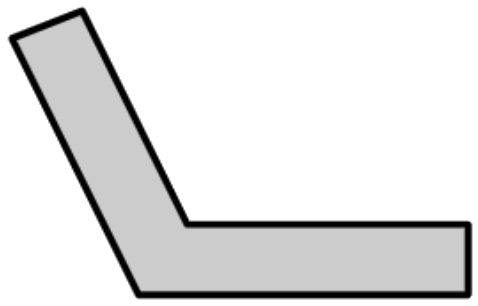
\includegraphics[width=0.6\columnwidth]{Figuras/fig20.png}
\end{center}

Haciendo la cuenta de $V, A, C$, obtenemos: $(V, A, C) = (12, 18, 10)$.



\textbf{ii) Una cabaña:}

\begin{center}
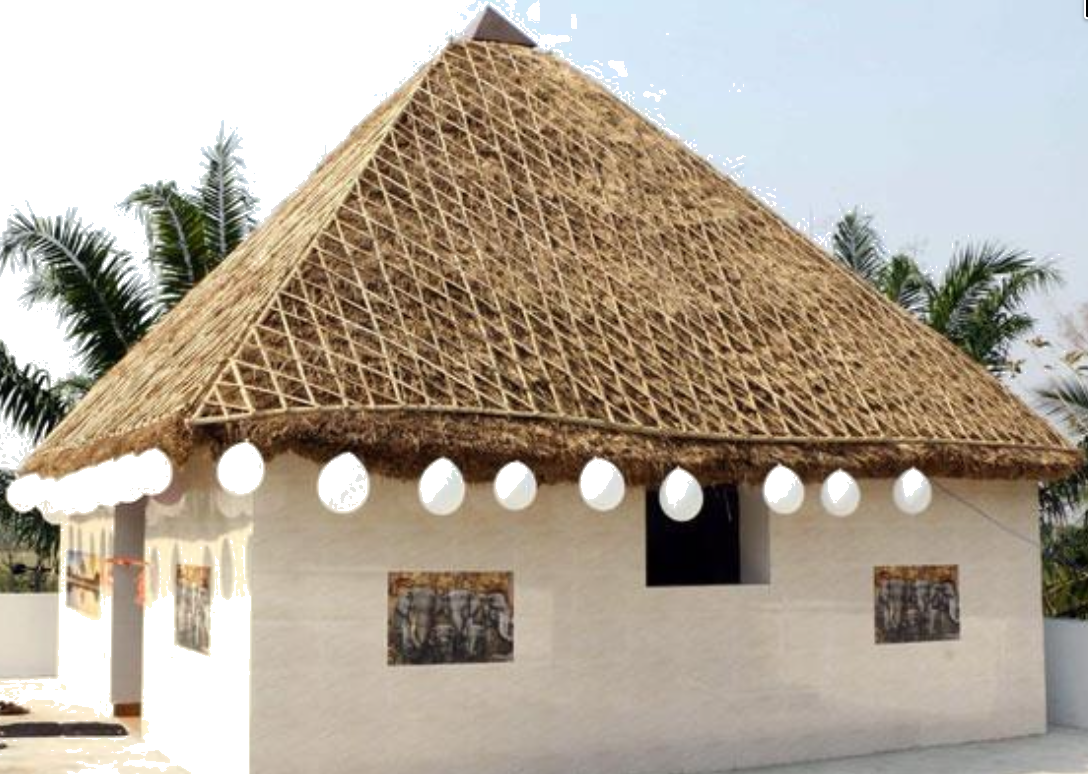
\includegraphics[width=0.65\columnwidth]{Figuras/fig21.png}
\end{center}

\textbf{Descomposición:} olvidándonos de puertas y ventanas, podemos descomponerla en dos sólidos: 
un ortoedro y una pirámide rectangular encima de él.

Recuerda que para el ortoedro, $(V, A, C) = (8, 12, 6)$. Para la pirámide rectangular tenemos 
$(V, A, C) = (5, 8, 5)$ (verifícalo).

De nuevo, el volumen de la cabaña se halla sumando los volúmenes de cada pieza. Para el área superficial, 
hay que sumar las áreas de cada sólido y luego restar dos veces la cara común rectangular.

\textbf{iii) Una caperuza de una lámpara:}

\begin{center}
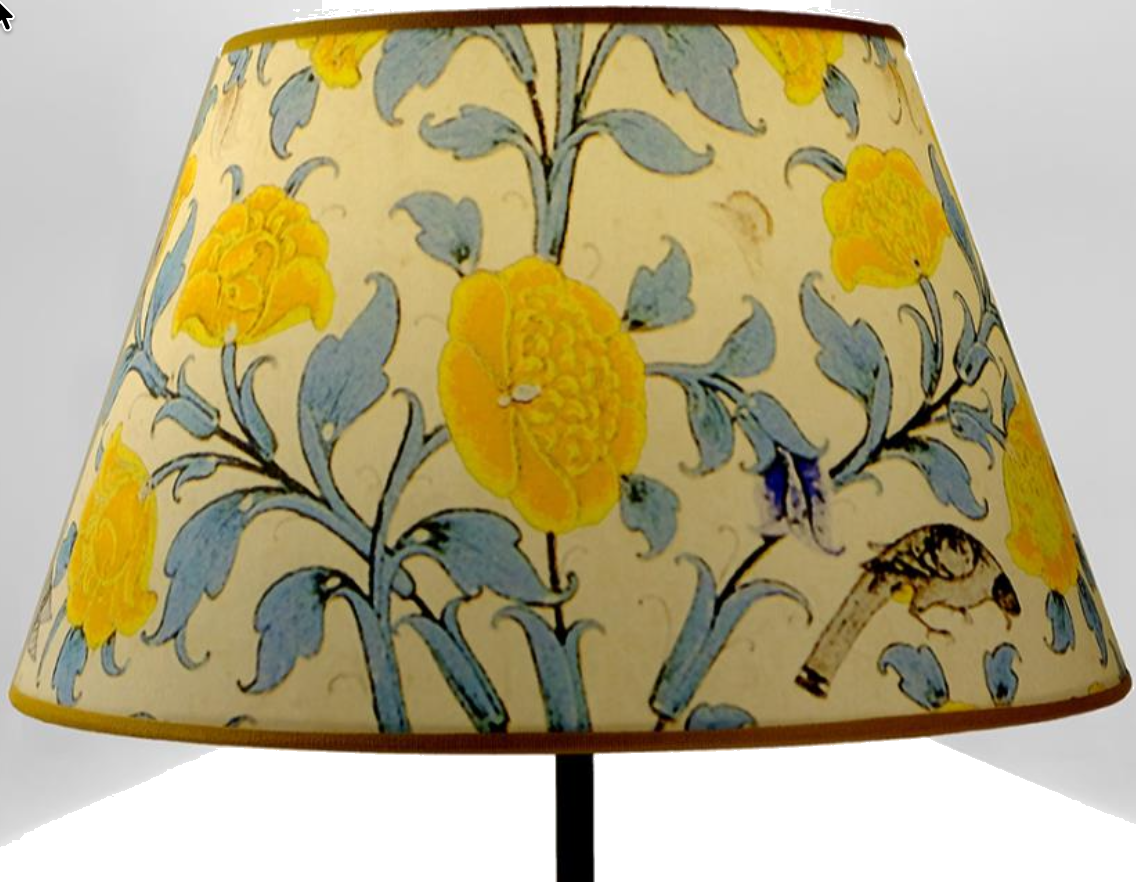
\includegraphics[width=0.75\columnwidth]{Figuras/fig22.png}
\end{center}

\textbf{Descomposición:} Una forma es usar una ``caneca'', es decir un cilindro circular. Entre menos angulada sea la caperuza, mejor será la aproximación. Además podemos aproximar ``por afuera'', cubriendo la caperuza (obtendremos más volumen del real), o ``por adentro'' de la caperuza, obteniendo menos volumen.

\textbf{Otra descomposición:} Una descomposición más precisa (de hecho, exacta) para la caperuza es usar un cono, cortarlo en 2, y eliminar la parte que tiene el vértice (que es también un cono. Esto es lo que se llama \textbf{CONO TRUNCADO} y es exactamente la forma de la caperuza.

Así: CONO GRANDE = CONO PEQUEÑO + CONO TRUNCADO.

Sabiendo cómo calcular el volumen de un cono usando radio y altura, esto nos permite calcular el volumen de la caperuza, restando los volúmenes de los conos.

\begin{tcolorbox}[colback=fondorosa, colframe=rojoclaro, breakable]
No es necesario memorizar la fórmula de volumen del cono truncado, ya que este lo puedes hallar usando la fórmula del volumen del cono ($V = \frac{1}{3}\pi r^2 h$). Usando proporcionalidad podrás hallar el radio del círculo donde empatan el cono truncado y el cono pequeño.
\end{tcolorbox}

Además, la altura del cono grande es igual a la altura del cono pequeño más la altura del cono truncado.

%\end{multicols}

\vspace{4mm}

%\begin{multicols}{2}

\textbf{iv) Un iglú:}

\begin{center}
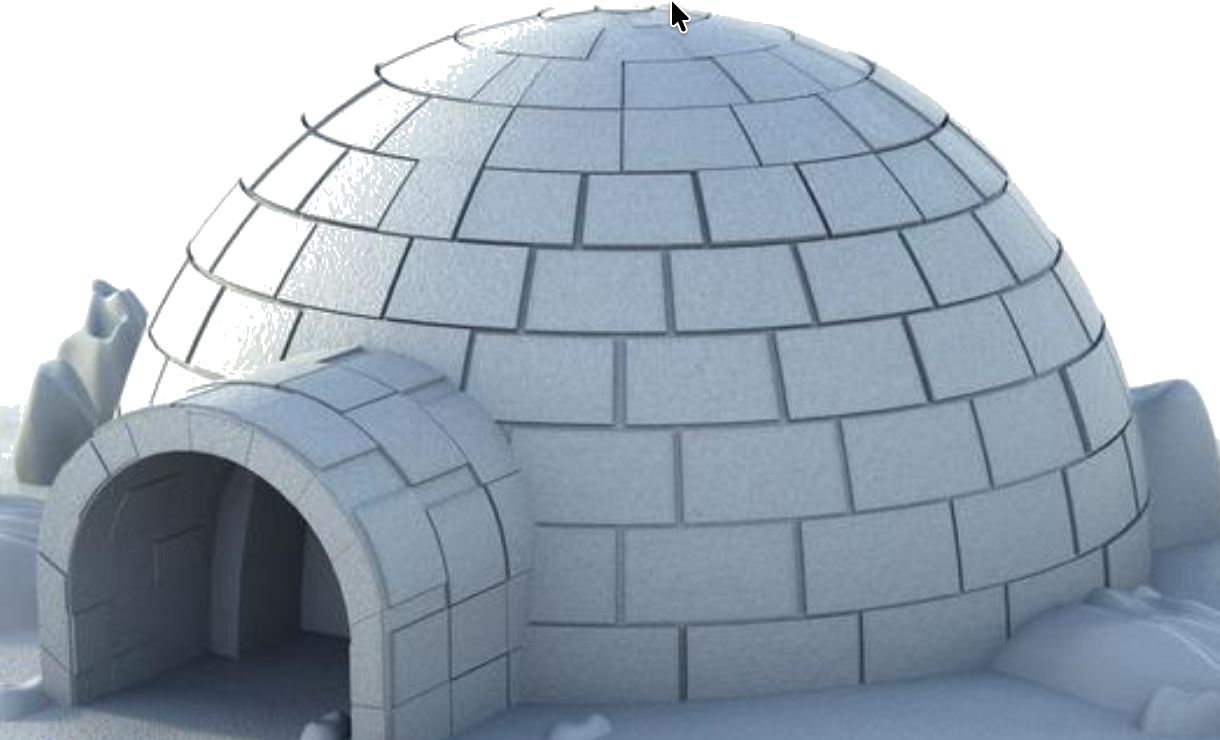
\includegraphics[width=0.7\columnwidth]{Figuras/fig25.png}
\end{center}

\textbf{Descomposición:} Aproximando un poco, podemos pensar que el iglú se descompone en 4 sólidos:

\begin{center}
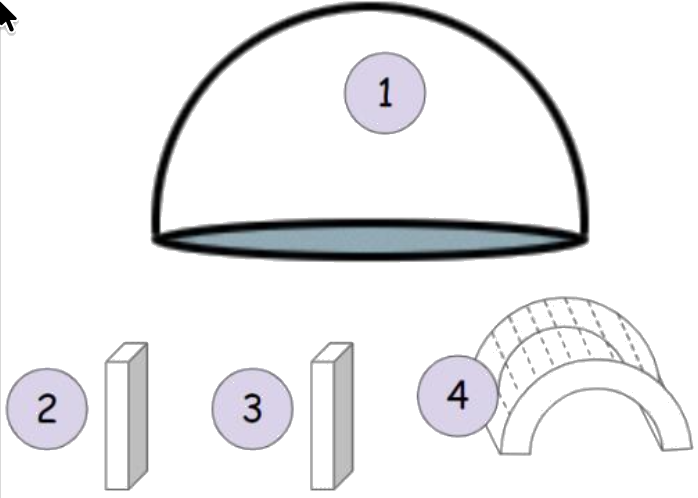
\includegraphics[width=0.75\columnwidth]{Figuras/fig26.png}
\end{center}

\begin{itemize}[nosep]
    \item Media esfera (es decir, un sólido en forma de hemisferio).
    \item 2 ortoedros, que forman parte de la entrada (los lados).
    \item Media ``cáscara'' cilíndrica de cierto grosor, similar a media caneca circular, que forma la parte de arco de la entrada. A esta figura la llamamos medio casquete cilíndrico. Es el análogo 3D de medio anillo 2D.
\end{itemize}

A partir de esto podemos encontrar el volumen y área superficial.

\begin{tcolorbox}[colback=fondorosa, colframe=rojoclaro, breakable]
No es necesario memorizar la fórmula de volumen de un casquete (cilíndrico), ya que este lo puedes hallar usando la fórmula del volumen del cilindro ($V = \pi r^2 h$). El casquete se obtiene al quitar un cilindro pequeño a uno más grande:

CASQUETE = CILINDRO GRANDE $-$ CILINDRO PEQUEÑO.

Así, si hacemos la resta de volúmenes, podremos hallar el volumen del casquete.
\end{tcolorbox}

\subsubsection*{Responde:}

\textbf{a)} Supongamos que el sofá (i) es reclinable (se cierra todo, 0 grados) y también es sofá cama (se abre completo, 180 grados). En cada situación, cómo cambia tu prototipo, el volumen y el área superficial con respecto a lo que se dijo antes? Explica.

\textbf{b)} Para calcular el área superficial y el volumen de un cubo basta con conocer la siguiente medida lineal: el largo de cualquiera de sus lados.

Para calcular el volumen de una pirámide, ¿qué medidas lineales necesitas conocer? Haz un dibujo con varias pirámides (de base triangular, cuadrada y rectangular no cuadrada).

\textbf{c)} Para cada uno de los sólidos i $-$ iv, haz una lista de las medidas lineales que necesitarías conocer para hallar el área superficial y el volumen de ellas. Además, averigua la fórmula si quieres, pero NO hagas cálculos (porque ni siquiera tenemos los datos).

\end{multicols}

\vspace{4mm}

%\newpage

\begin{tcolorbox}[colback=fondorosa, colframe=rojoclaro, title=\textbf{Mini-explicación: Descomponiendo un sólido usando otros sólidos}, breakable]
\textbf{DESCOMPONIENDO UN SÓLIDO USANDO OTROS SÓLIDOS}

\begin{multicols}{2}
	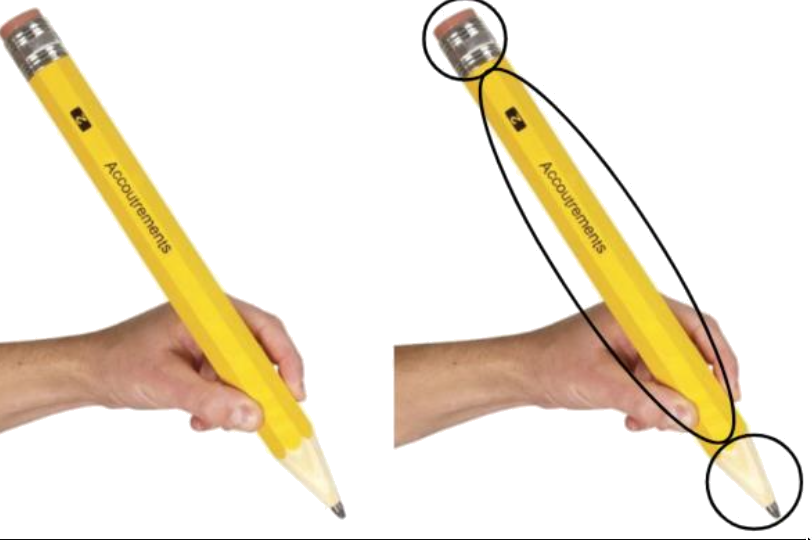
\includegraphics[width=\linewidth]{Figuras/fig27.png}
	
	%\columnbreak
En la vida real hay muchos sólidos complejos, que sin embargo pueden descomponerse en varios sólidos ``básicos'' (que conocemos bien y podemos hallar su volumen y área superficial, usando fórmulas que podemos consultar). A veces en esta descomposición aproximamos las formas sin perder mucha exactitud.

El volumen del sólido inicial será siempre igual a la suma de los volúmenes de cada sólido básico (o aproximadamente igual, si hicimos alguna aproximación de forma).

El área superficial es un poco más de cuidado: tenemos que tener en cuenta en qué cara se pegan los sólidos básicos para formar el sólido inicial, y no contar el área de esa cara para el área superficial.

Por ejemplo, podríamos aproximar este lápiz usando un cilindro circular y un cono, o aún mejor:

\vspace{3mm}

\begin{itemize}[nosep, leftmargin=*]
  \item Un cilindro circular (borrador).
  \item Un prisma hexagonal (cuerpo).
  \item Un cono (punta).
\end{itemize}
\end{multicols}

\vspace{2mm}
\end{tcolorbox}

\vspace{4mm}

%\newpage

\subsubsection*{Paso 1: Ejemplo: Aproximando medio hemisferio}

\begin{wrapfigure}{r}{0.4\textwidth}
\centering
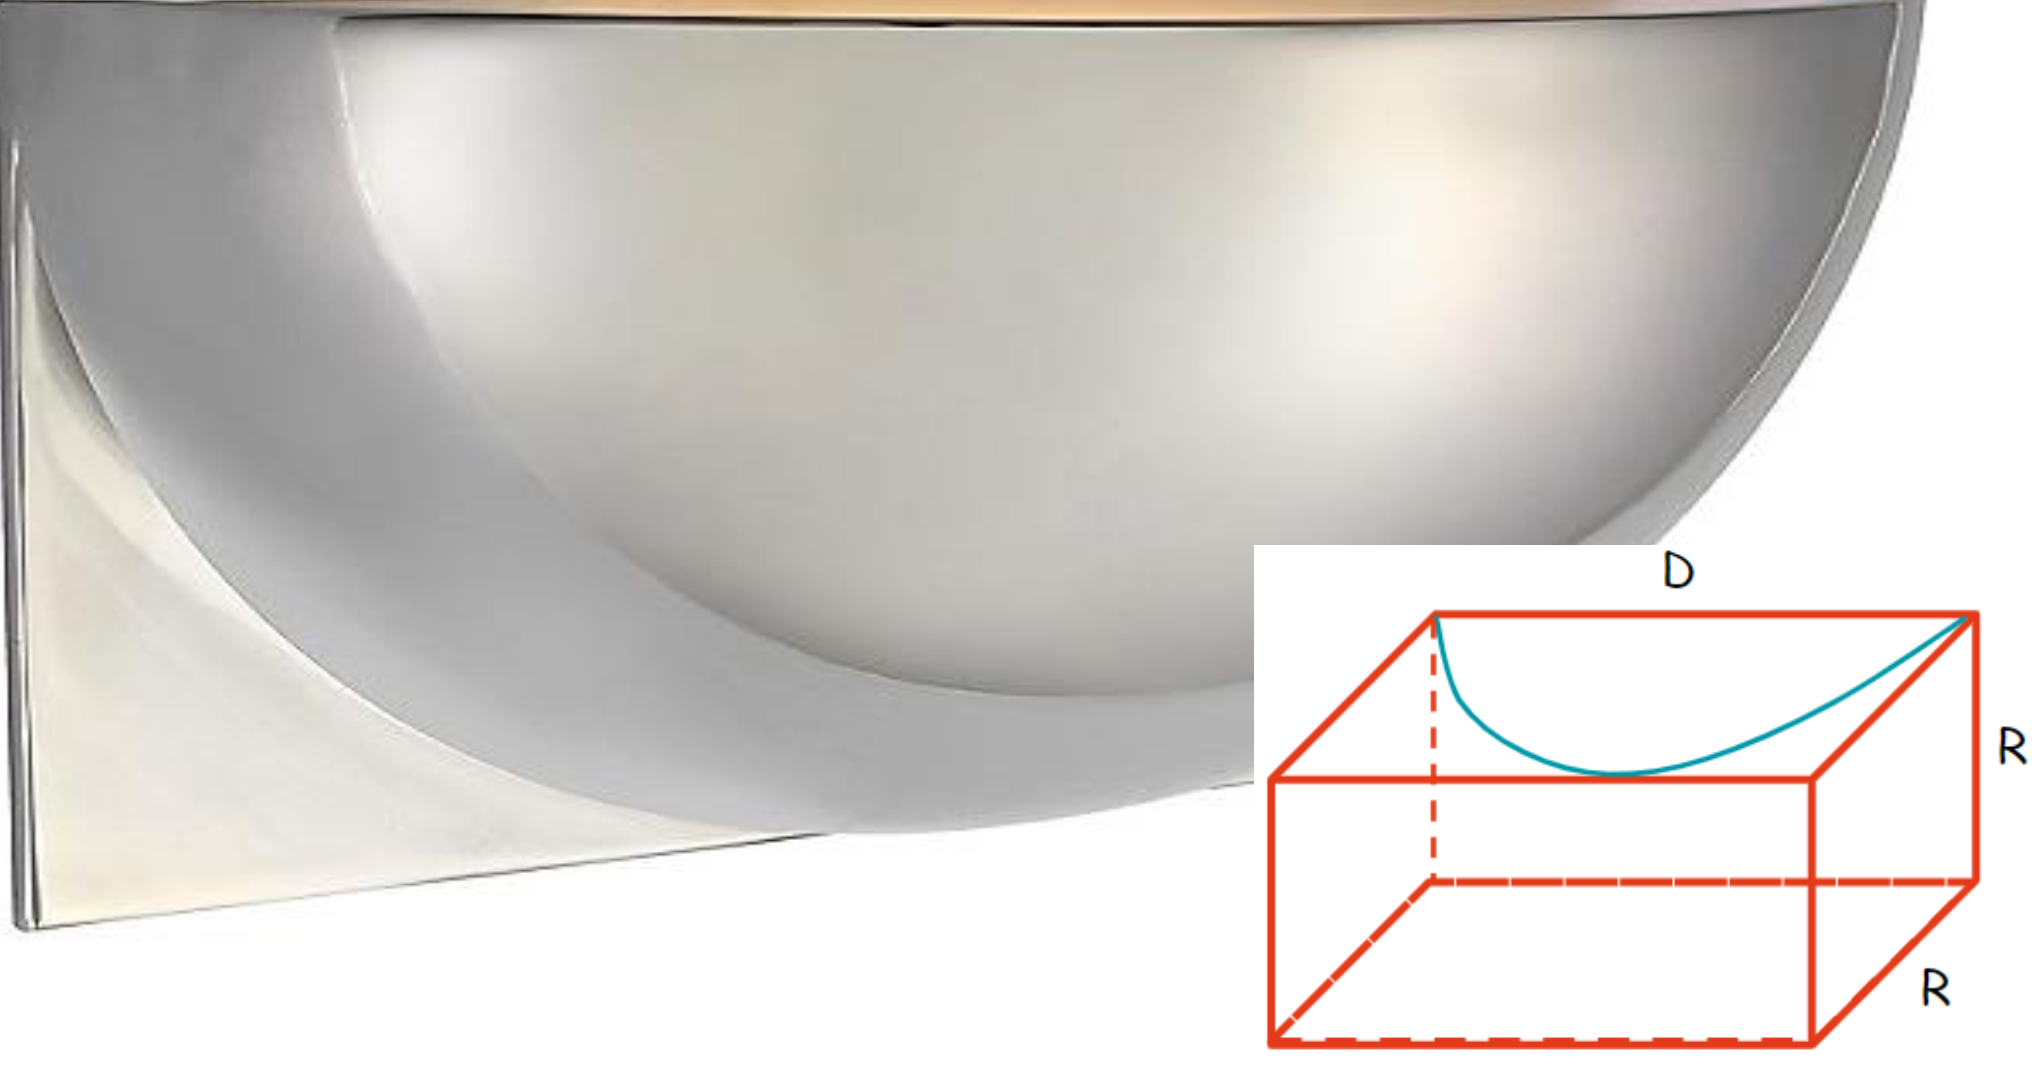
\includegraphics[width=0.38\textwidth]{Figuras/fig29a.png}
\end{wrapfigure}

Una diseñadora del Meta quiere elaborar un lavamanos en forma de medio hemisferio, es decir, de un cuarto de esfera, como puedes ver.

Para su primer prototipo desea trabajar únicamente con poliedros, es decir, sólidos con caras que no son curvas, sino que son polígonos, o con conos.

¿Cómo puede la diseñadora hacer su prototipo?

Para cada opción de prototipo, ¿qué tan buena es la aproximación del volumen?

\textbf{Solución:}

\textbf{i)} Intentemos primero con un ortoedro (es decir, ``cilindro recto rectangular'' o caja), que aproxime el lavamanos por afuera, es decir, que lo contenga.

\begin{tcolorbox}[colback=fondoverde, colframe=verdeclaro]
\begin{wrapfigure}{r}{0.35\textwidth}
\centering
\vspace{-10pt}
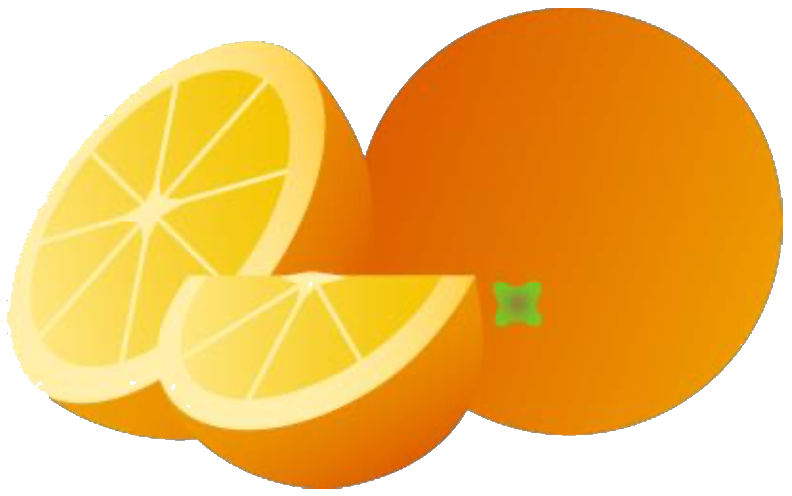
\includegraphics[width=0.23\textwidth]{Figuras/fig29b.png}
\vspace{-10pt}
\end{wrapfigure}

Si te está costando visualizar el lavamanos:
\begin{itemize}[nosep]
    \item Toma una naranja (u otra fruta esférica)
    \item Pártela en 2 y quédate con 1 hemisferio
    \item Parte el hemisferio en 2 y quédate con un pedazo.
\end{itemize}

¿Cuál es la menor caja que contiene ese pedazo?
\end{tcolorbox}

Usemos variables para las longitudes. Sea $R$ el radio del lavamanos y $D = 2R$ su diámetro. Entonces la caja tendría medidas $D$, $R$ y $R$. Es decir, $2R$, $R$ y $R$.

\begin{wrapfigure}{r}{0.35\textwidth}
\centering
\vspace{-5pt}
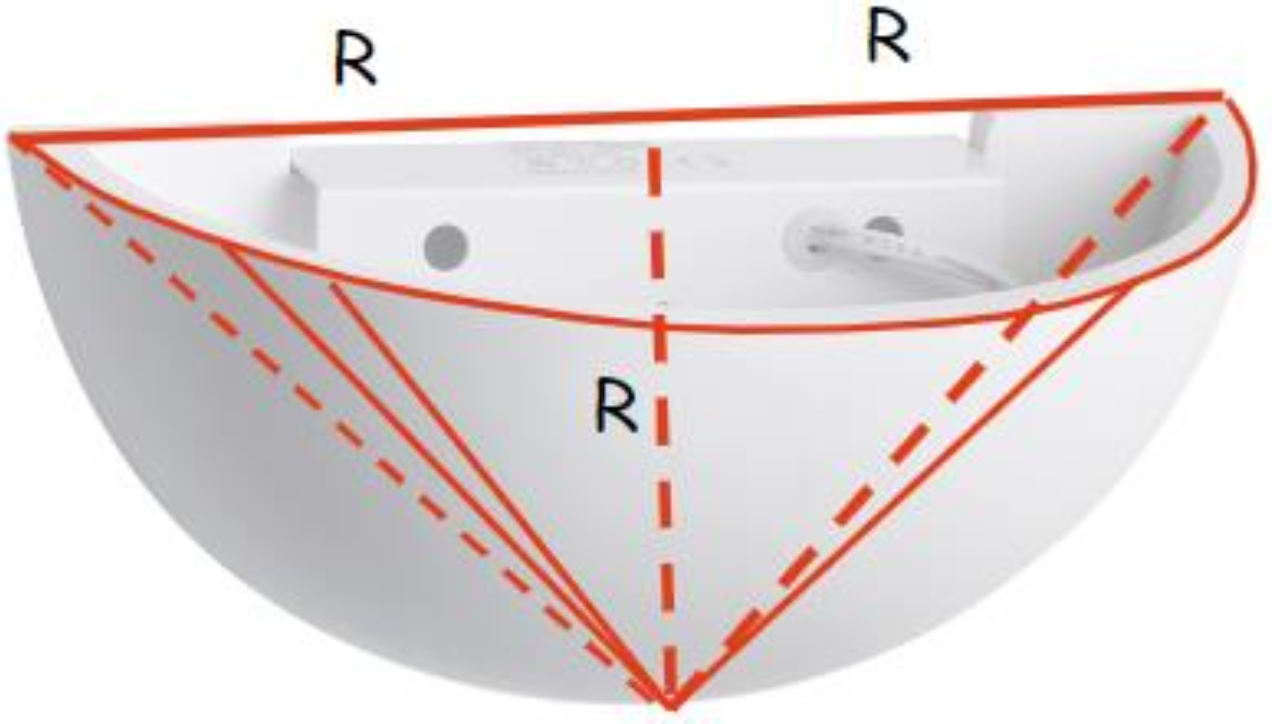
\includegraphics[width=0.33\textwidth]{Figuras/fig29c.png}
\vspace{-5pt}
\end{wrapfigure}

\textbf{Comparemos volúmenes:}

Una esfera con radio $R$ tiene un volumen igual a $\frac{4}{3}\pi R \times R \times R$, que es aproximadamente $4,2 R^3$. Así, un cuarto de esfera de radio $R$ tendrá aproximadamente $R^3$ de volumen (un poco más que eso).

La caja que proponemos es un ortoedro, así que su volumen es el producto LARGO $\times$ ANCHO $\times$ ALTO. En este caso es $2R \times R \times R = 2R^3$.

Así, nuestra aproximación no es buena. ¡Estamos duplicando el volumen!

\textbf{ii)} Intentemos ahora con un medio cono que aproxime el lavamanos por dentro, es decir, que esté contenido en el lavamanos.

\begin{wrapfigure}{r}{0.2\textwidth}
\centering
\vspace{-5pt}
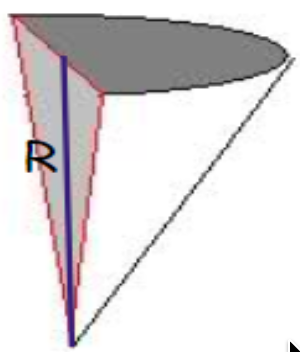
\includegraphics[width=0.17\textwidth]{Figuras/fig29d.png}
\vspace{-5pt}
\end{wrapfigure}

El cono está invertido (con la punta hacia abajo). La cara superior es medio círculo que empata perfecto con la parte superior del lavamanos.

La altura del medio cono es la misma del lavamanos, es decir, $R$.

\textbf{Comparemos volúmenes:}

Recordemos que el lavamanos mide cerca de $R^3$ en volumen. Recordemos que un cono de altura $H$ y base circular de radio $R$ tiene el siguiente volumen: $\frac{1}{3}\pi R \times R \times H$. En este caso $H = R$ y estamos usando medio cono, entonces su volumen es igual a $(\frac{1}{3}\pi R \times R \times R)/2 = \frac{1}{6}\pi R^3$, es decir, un poco más de $0,5 R^3$ (dado que $\pi$ es un poco más de 3).

Esta estimación es muy poco cercana del volumen real del lavamanos. ¡Sólo llenaríamos la mitad del agua!

\textbf{Reto:} ¿puedes pensar en otro sólido que pueda aproximar mejor el volumen del lavamanos?

\vspace{4mm}

%\newpage

\subsubsection*{Paso 2: Completa este ejemplo: ¿Qué porcentaje se llena?}

\begin{wrapfigure}{r}{0.35\textwidth}
\centering
\vspace{-5pt}
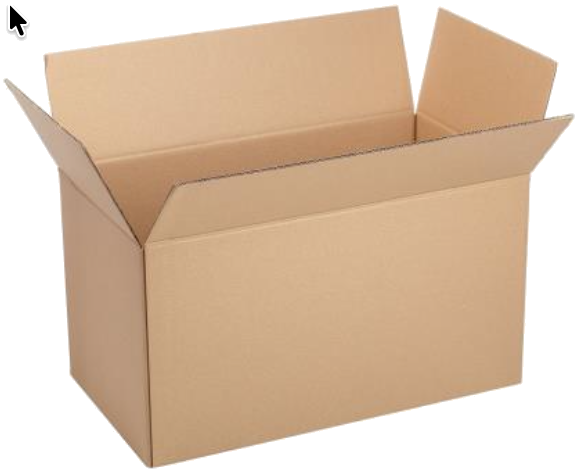
\includegraphics[width=0.33\textwidth]{Figuras/fig31.png}
\vspace{-5pt}
\end{wrapfigure}

Claudia va a empacar un sólido grande en una caja y a rellenar lo que sobre con aserrín. Los objetos caben JUSTO en la caja. Es decir, ninguna caja de menor volumen podría contenerlos. Lo que queremos es decidir, para cada objeto, qué porcentaje de la caja realmente se llena.

Las dimensiones de la caja son, en decímetros: $2 \times 4 \times 6$.

\textbf{a)} Una esfera: Esta debe ser de radio igual a 1 dm. Justifica por qué.

Luego su volumen es igual a $\frac{4}{3}\pi R^3 = \frac{4}{3}\pi 1^3 \approx 4,2$ dm. Halla la proporción de volumen de la caja que la esfera ocupa y haz un dibujo.

\textbf{b)} Una pirámide rectangular con un rectángulo de 2 por 6 (en decímetros) de base. Halla la proporción de volumen que ocupa. [Recuerda que la pirámide es tan alta como se puede para que quepa en la caja.]

\textbf{c)} Completa la siguiente tabla que incluye los objetos anteriores con unos nuevos. Aproxima volúmenes (recuerda que $\pi \approx 3,1$) y recuerda que los sólidos deben caber en la caja y ser lo más grandes posibles.

\begin{center}
\small
\begin{tabular}{|
		>{\centering\arraybackslash}m{2.2cm}|
		>{\centering\arraybackslash}m{3.2cm}|
		>{\centering\arraybackslash}m{3.5cm}|
		>{\centering\arraybackslash}m{2cm}|
		>{\centering\arraybackslash}m{1.5cm}|}
\hline
\textbf{Sólido} & \textbf{Información adicional} & \textbf{Volumen (fórmula)} & \textbf{Vol. aprox. (dm$^3$)} & \textbf{\% caja} \\
\hline
Esfera \newline 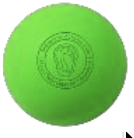
\includegraphics[width=2cm]{Figuras/fig32.png} & Ninguna & $V = \frac{4}{3}\pi R^3$ ($R$ = radio) & 4,2 & 8,8\% \\
\hline
Pirámide rectangular \newline 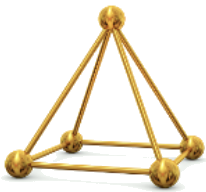
\includegraphics[width=2cm]{Figuras/fig33.png} & Base: rectángulo 2 dm $\times$ 6 dm & $V = \frac{1}{3}XYZ$ Base: $X \times Y$. Altura: $Z$ & ? & ? \\
\hline
Cono \newline 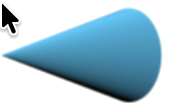
\includegraphics[width=2cm]{Figuras/fig34.png} & Altura: 2 dm & ? & ? & ? \\
\hline
Prisma triangular & Área base triangular: 12 dm$^2$ & ? & ? & ? \\
\hline
\end{tabular}
\end{center}

\vspace{5mm}

%\newpage

\subsubsection*{Paso 3: Tu turno: ¿Qué porcentaje del cubo se llena?}

\begin{wrapfigure}{l}{0.25\textwidth}
\centering
\vspace{-5pt}
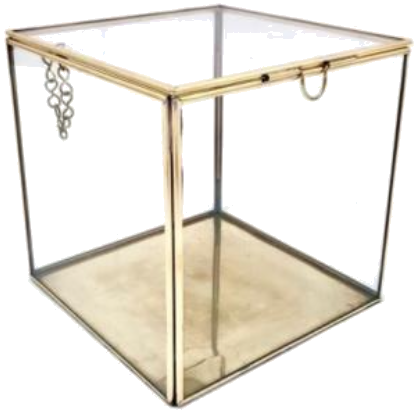
\includegraphics[width=0.23\textwidth]{Figuras/fig35.png}
\vspace{-5pt}
\end{wrapfigure}

Tienes un cubo de lado $X$ m. Quieres hacer lo mismo que en el Paso 2, es decir, pensar en objetos tan grandes como se puedan que quepan dentro del cubo, pero ahora quieres estimar el espacio del cubo que NO se llena.

Elabora una tabla como la del Paso 2, con 4 distintos objetos (puedes repetir algunos del Paso 2, pero intenta también incluir nuevos tipos de objetos).

Recuerda hacer un dibujo en cada situación para verificar visualmente que el porcentaje de ``no llenado'' es razonable. Prepárate para explicarle a tu profesor.

\begin{tcolorbox}[colback=fondorosa, colframe=rojoclaro, title=\textbf{PROYECTO GRUPAL - APLIQUEMOS LO APRENDIDO}, breakable]
Formen grupos de 4 estudiantes. Vamos a trabajar en un proyecto para aplicar lo que aprendimos.

\textbf{Instrucciones:}

\begin{enumerate}[nosep]
    \item Elijan un sólido que les llame la atención de la vida real. No puede ser muy simple (no puede ser un cubo, ni una esfera, etc), pero tampoco elijan un sólido demasiado irregular. Busquen un punto medio. Si tienen el sólido a la vista, mucho mejor. Si no, al menos tengan una imagen o fotografía.

    \item Describan cómo lo pueden descomponer en 2 o más sólidos básicos, y digan si deben hacer una aproximación. Estimen el porcentaje de error, relativo al volumen real del sólido.

    \item Identifiquen todas las medidas lineales que necesitarían para calcular o estimar el volumen del sólido (longitudes, diámetros, alturas, circunferencias, etc). Especifiquen la mejor unidad de medida (cm, m, km, etc.).

    \item Describan cómo hallarían el área superficial de cada pieza, y la del sólido inicial.

    \item Cuenten las Caras, Aristas y Vértices de los sólidos base, si es que eran poliedros.
\end{enumerate}
\end{tcolorbox}

\vspace{4mm}

%\newpage

\subsection*{C) Resuelve y practica}

\setlength{\columnseprule}{0.4pt}
\begin{multicols}{2}

\textbf{1)} Para cada uno de estos sólido geométricos, determina si es un poliedro o un cuerpo redondo, e identifica varios objetos comunes que tengan una forma parecida.

\begin{itemize}[nosep]
    \item Una esfera
    \item Un ortoedro
    \item Un cilindro circular
    \item Un cono
    \item Una pirámide truncada
    \item Un prisma triangular
\end{itemize}

\textbf{2)} Considera los siguientes 8 sólidos:

\begin{itemize}[nosep]
    \item Un cubo
    \item Un tetraedro
    \item Un cono truncado
    \item Un hemisferio
    \item Una pirámide de base circular
    \item Un cilindro circular
    \item Un cilindro hexagonal
    \item Un casquete cilíndrico
\end{itemize}

\textbf{a)} Haz un dibujo de cada sólido. Puedes pedir ayuda si tienes dudas.

\textbf{b)} Invéntate una forma propia de clasificar estos sólidos en 3 categorías distintas y disjuntas. Tienes toda la libertad para formar tus categorías, pero defínelas muy bien.

\textbf{c)} Un prisma triangular, ¿a qué categoría pertenecería? ¿Alguna de las 3, o pertenecería a una nueva categoría?

\textbf{d)} Ordena los 8 sólidos en orden creciente de dificultad (en tu opinión) para calcular su volumen. Justifica tu ordenamiento.

\textbf{3)} Para cada uno de los siguientes objetos:

\begin{itemize}[nosep]
    \item Indica cómo descomponerlo en 2 más sólidos básicos, cómo verlo como una fracción de un sólido básico, o decide que ya se puede ver como sólido básico.
    \item Indica si estás haciendo alguna aproximación de forma, o si solo estás haciendo una descomposición. Dí qué tan buena, en tu opinión, es tu aproximación.
\end{itemize}

\textbf{f)} Octaedro

\begin{center}
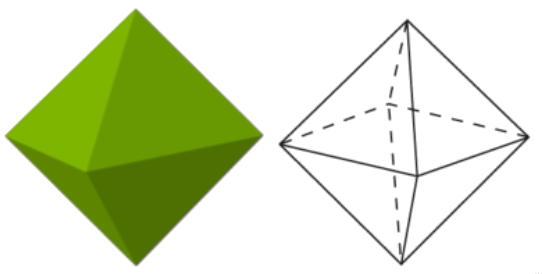
\includegraphics[width=0.75\columnwidth]{Figuras/fig39.png}
\end{center}

\textbf{g)} Aguacate partido por la mitad

\begin{center}
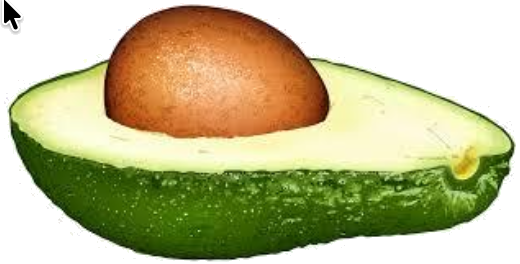
\includegraphics[width=0.75\columnwidth]{Figuras/fig40.png}
\end{center}

\textbf{h)} Punta de flecha

\begin{center}
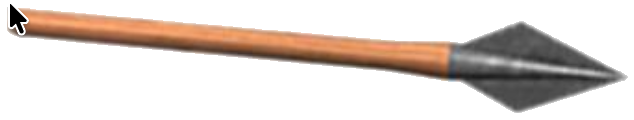
\includegraphics[width=0.75\columnwidth]{Figuras/fig41.png}
\end{center}

\textbf{4)} Una caja de cubitos de azúcar trae 320 cubos de 1 cm$^3$. Propón posibles dimensiones para las cajas, sabiendo que no quedan espacios vacíos.

\vspace{4mm}

%\newpage

\textbf{5)} De los siguientes cuerpos, di cuáles son poliedros y cuáles no. Explica tus razones.
\begin{center}
	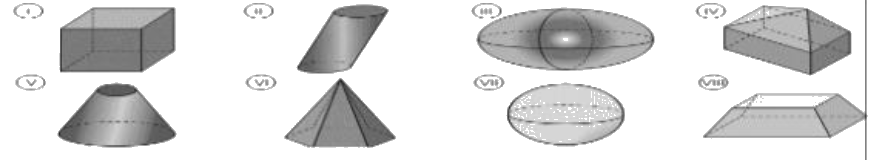
\includegraphics[width=0.75\columnwidth]{Figuras/fig46.png}
\end{center}

 \textbf{Los sólidos platónicos}  \\
Los sólidos platónicos son \textbf{CONVEXOS}. Esto significa que si trazamos una recta imaginaria entre dos puntos dentro del sólido, la recta nunca se sale del sólido (algo similar ocurre con una esfera, pero no con una donut, por ejemplo.)

El filósofo Platón, en su diálogo Timaeus, asoció cada sólidos platónicos a una cosa distinta: fuego al tetraedro (4), tierra al cubo (hexaedro, 6), aire al octaedro (8), el universo al dodecaedro (12) y agua al icosaedro (20).

\textbf{6)}  ¿Qué tienen en común los números 4, 6, 8, 12 y 20? Estas son las distintas cantidades de caras de los llamados \textbf{SÓLIDOS PLATÓNICOS}, que son sólidos cuyas caras son polígonos regulares.

\textbf{a)} Para cada sólido platónico, contemos cuántos vértices, aristas y caras tiene. Para eso, completa esta tabla que relaciona distintas dimensiones (3D, 2D, 1D, 0D):

\begin{center}
\small
\begin{tabular}{|
		>{\centering\arraybackslash}m{2.7cm}|
		>{\centering\arraybackslash}m{1.2cm}|
		>{\centering\arraybackslash}m{1.2cm}|
		>{\centering\arraybackslash}m{1.2cm}|}
\hline
\textbf{Sólido platónico} & \textbf{C (2D)} & \textbf{A (1D)} & \textbf{V (0D)} \\
\hline
Tetraedro \newline 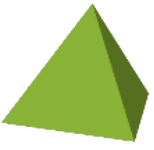
\includegraphics[width=1.7cm]{Figuras/fig43.png} & 4 & 6 & 4 \\
\hline
Cubo (Hexaedro) \newline 
\includegraphics[width=1.7cm]{Figuras/fig44.png} & 6 & ? & 8 \\
\hline
Octaedro \newline 
\includegraphics[width=1.7cm]{Figuras/fig45.png} & 8 & 12 & ? \\
\hline
Dodecaedro \newline 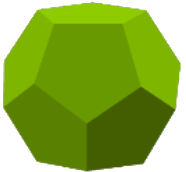
\includegraphics[width=1.7cm]{Figuras/fig47.png} & ? & ? & ? \\
\hline
Icosaedro \newline 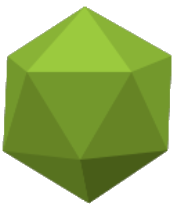
\includegraphics[width=1.7cm]{Figuras/fig48.png} & ? & ? & ? \\
\hline
\end{tabular}
\end{center}

\textbf{b)} El \textbf{Teorema de Euler} para poliedros convexos nos dice que para estos sólidos se cumple una relación:

\begin{center}
\underline{\hspace{1cm}} + \underline{\hspace{1cm}} $-$ \underline{\hspace{1cm}} = \underline{\hspace{1cm}}
\end{center}

Usando la tabla en a), llena los cuatro espacios con $A$, $C$, $V$ y un número (descúbrelo) en el orden correcto... ¡ensaya! Debes encontrar una única fórmula que sirva en TODOS los casos (por eso se llama Teorema, es un resultado general).

Si quieres profundizar en este apasionante tema, consulta el siguiente enlace: \url{https://es.wikipedia.org/wiki/Característica_de_Euler}
\vspace{5mm}
%\newpage

\textbf{7)} Expresa el volumen de cada sólido en términos de la variable $X$. Todas las medidas están en cm y el sólido B es un cubo.

\begin{center}
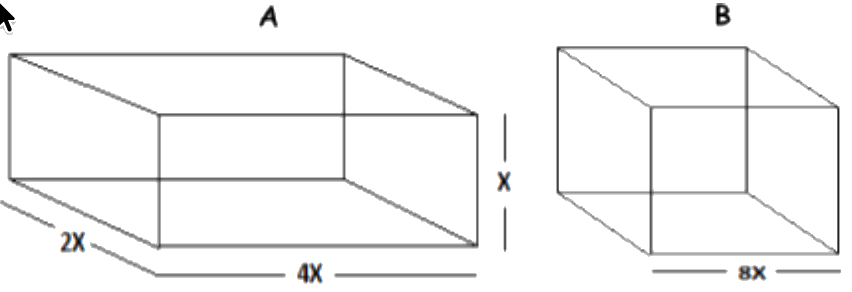
\includegraphics[width=0.9\columnwidth]{Figuras/fig51.png}
\end{center}

\textbf{8)} \textbf{Afianza tus habilidades de cálculo en relación con volúmenes:}

Elige algunos de estos ejercicios, según necesites practicar procedimientos para encontrar volúmenes.

\textbf{a)} Las dimensiones de una piscina en forma de paralelepípedo son: 45 m de larga, 30 m de ancha y 2 m de profunda. Calcula cuánta agua contiene si solo se llena hasta la mitad.

\textbf{b)} Halla la altura de un tanque cilíndrico circular de 3000 litros de capacidad y diámetro de la base 10 m.

\textbf{c)} ¿Qué sólido tiene más volumen?
\begin{itemize}[nosep]
    \item un cubo de lado 2 m.
    \item un cilindro circular de altura 3 m y radio 1 m.
    \item una pirámide de altura 7 m y base cuadrada de 2 m por 2 m. (Dibuja los tres sólidos y conjetura tu respuesta antes de hacer los cálculos)
\end{itemize}

\begin{wrapfigure}{r}{0.35\columnwidth}
	\centering
	\vspace{-10pt}
	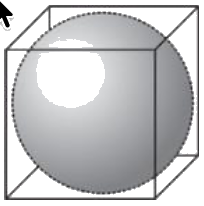
\includegraphics[width=0.3\columnwidth]{Figuras/fig50.png}
	\vspace{-10pt}
\end{wrapfigure}
\textbf{d)} Calcula el volumen de la esfera de madera más grande que puede ser tallada a partir de un bloque cúbico de 12 cm de arista.

\vspace{2mm}

\textbf{e)} Calcula el volumen de la gasolina contenida en la caneca de la siguiente figura si está llena hasta la mitad.

\begin{center}
\begin{tikzpicture}[scale=0.8]
% Caneca cilíndrica con gasolina
% Base inferior
\draw[thick, fill=gray!20] (0,0) ellipse (1.5 and 0.4);
% Cuerpo del cilindro
\draw[thick] (-1.5,0) -- (-1.5,4);
\draw[thick] (1.5,0) -- (1.5,4);
% Gasolina hasta la mitad
\fill[yellow!60, opacity=0.7] (-1.5,0) -- (-1.5,2) arc (180:360:1.5 and 0.4) -- (1.5,0) arc (360:180:1.5 and 0.4);
\draw[thick, dashed] (-1.5,2) arc (180:360:1.5 and 0.4);
% Tapa superior
\draw[thick, fill=gray!20] (0,4) ellipse (1.5 and 0.4);
% Dimensiones
\draw[<->, red, thick] (2,0) -- (2,4) node[midway, right] {$h = 80$ cm};
\draw[red, thick] (0,0) -- (1.5,0) node[midway, above] {$r = 25$ cm};
% Nivel de gasolina
\draw[<->, blue, thick] (-2.2,0) -- (-2.2,2) node[midway, left] {Mitad};
\end{tikzpicture}
\end{center}

\textbf{f)} Dibuja el modelo de dos pirámides rectangulares diferentes cuyo volumen sea 384 m$^3$. Asigna las medidas a las dimensiones.

\textbf{g)} Se coloca un bloque en forma de ortoedro, con base cuadrada y altura 10 cm dentro de un cilindro de igual altura y de radio 6 cm. Determine el área total y el volumen del bloque. ¿Cuál es el volumen de la porción del cilindro que queda vacía?

\textbf{i)} Calcula la altura de una pirámide de base cuadrada de 169 cm$^2$ de área y volumen 2028 cm$^3$.

\textbf{j)} Calcula el volumen de una pirámide triangular cuya base es un triángulo equilátero de 1 m de lado y la altura mide 1m. [Ayuda: recuerda cómo calcular el área de un triángulo equilátero si conocemos su lado.]

\vspace{5mm}

 \begin{wrapfigure}{r}{0.35\columnwidth}
\centering
\vspace{-25pt}
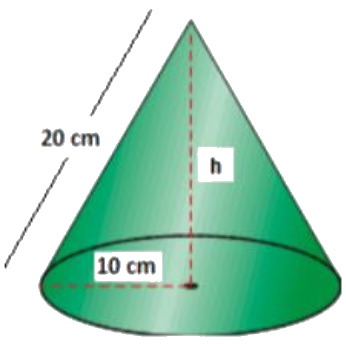
\includegraphics[width=0.3\columnwidth]{Figuras/fig52.png}
\vspace{-20pt}
\end{wrapfigure}
\textbf{k)} Calcula el volumen de un cono cuya generatriz (su ``diagonal'') mide 20 cm y el radio de su base es 10 cm.

\vspace{5mm}

\textbf{9)} \textbf{Práctica en GeoGebra:}

Ingresa al enlace: \url{www.geogebra.org/m/tf2IohN0} y después de practicar con el programa GeoGebra, usa tus conocimientos y haz la Actividad 1 de dicha página. Le puedes preguntar a tu maestro sobre el programa. La actividad deber ser entregada.

\end{multicols}

\vspace{4mm}

%\newpage

\subsection*{D) Resumen}

\begin{center}
\textbf{SÓLIDOS}

$\downarrow$

Puede incluir aproximaciones en formas

$\downarrow$

Descomponer en varias piezas básicas

$\downarrow$

Usarlas para encontrar

$\swarrow$ \hspace{3cm} $\searrow$

\textbf{VOLUMEN} \hspace{2cm} \textbf{ÁREA DE SUPERFICIE}
\end{center}

\begin{tcolorbox}[colback=fondoazul, colframe=azuloscuro, title=\textbf{VOLUMEN}, breakable]
\begin{center}
\begin{tabular}{|
		>{\centering\arraybackslash}m{3.5cm}|
		>{\centering\arraybackslash}m{3.5cm}|
		>{\centering\arraybackslash}m{3.5cm}|}
\hline
\textbf{Cilíndricos} & \textbf{Puntiagudos} & \textbf{Esféricos} \\
\hline
\textbf{Prisma}

En particular, cubos, ortoedros

Volumen: se multiplica el área de la base por la altura. &
\textbf{Pirámide}

En particular, tetraedro, pirámide rectangular

Volumen: un tercio del volumen del prisma más pequeño que la contendría. &
\textbf{Esfera y hemisferio} (``Pelotas'')

Volumen de una esfera de radio $R$:
$$\frac{4}{3}\pi R \times R \times R$$ \\
\hline
\textbf{Cilindro circular}

(Base circular)

Volumen: se multiplica el área de la base por la altura. &
\textbf{Cono}

Volumen: un tercio del volumen del cilindro circular más pequeño que lo contendría. & \\
\hline
\end{tabular}
\end{center}
\end{tcolorbox}

\begin{tcolorbox}[colback=fondoverde, colframe=verdeclaro, title=\textbf{Ten en cuenta que:}, breakable]
\begin{itemize}[nosep]
    \item Hay distintas formas de descomponer un sólido y algunas serán más convenientes que otras. La práctica hace al maestro.
    \item Los prismas y cilindros circulares tienen la misma forma para hallar su volumen: multiplicar el área de la base por la altura.
    \item La fórmulas de volumen del cilindro y el cono son muy parecidas; la del cono es la tercera parte de la del cilindro (con mismo radio de la base y altura).
    \item Las pirámides y conos truncados tienen un volumen que se puede calcular restando volúmenes de dos pirámides o dos conos respectivamente. No es necesario aprender de memoria las fórmulas de volumen de los conos y pirámides truncadas.
    \item La fórmula del volumen implica que una esfera de radio $R$ ocupa aproximadamente la mitad del volumen del mínimo cubo que la contiene (de lado 2$R$). Es importante tener este sentido de proporción.
\end{itemize}
\end{tcolorbox}

\vspace{4mm}

%\newpage

\subsection*{E) Valoración}

\textbf{i) Califica tu comprensión por tema en tu cuaderno}

\begin{center}
\small
\begin{tabular}{|
		>{\centering\arraybackslash}m{5.5cm}|
		>{\centering\arraybackslash}m{2.5cm}|
		>{\centering\arraybackslash}m{2.5cm}|
		>{\centering\arraybackslash}m{2.5cm}|}
\hline
\textbf{Tema} & \textbf{$\bullet\circ\circ$ No entiendo (TODAVÍA)} & \textbf{$\bullet\bullet\circ$ Voy bien} & \textbf{$\bullet\bullet\bullet$ Comprendí bien} \\
\hline
Descompongo un sólido en otros sólidos básicos & & & \\
\hline
Razono para hallar el volumen de una pirámide & & & \\
\hline
Razono para hallar el volumen de un cono & & & \\
\hline
Razono para hallar el volumen de una esfera & & & \\
\hline
\end{tabular}
\end{center}

\textbf{ii) Preguntas de comprensión}

\textbf{1)} Si cada lado de un cubo se triplica, entonces el volumen del cubo...

[ ] se multiplica por 3.

[ ] se multiplica por 27.

\textbf{2)} Si la altura de un cono se duplica, entonces el volumen del cono...

[ ] se multiplica por 2.

[ ] se multiplica por 8.

\textbf{3)} Si el radio de la base de un cono se triplica, entonces el volumen del cono...

[ ] se multiplica por 3.

[ ] se multiplica por 9.

\textbf{4)} Si el volumen de una esfera se reduce a 1/8, entonces el radio...

[ ] se reduce a 1/2.

[ ] se reduce a 1/512.

(Verifica las respuestas con tu profesor)

\vspace{4mm}

%\newpage

\textbf{iii) Resuelvo un problema}

\begin{wrapfigure}{r}{0.28\textwidth}
\centering
\vspace{-20pt}
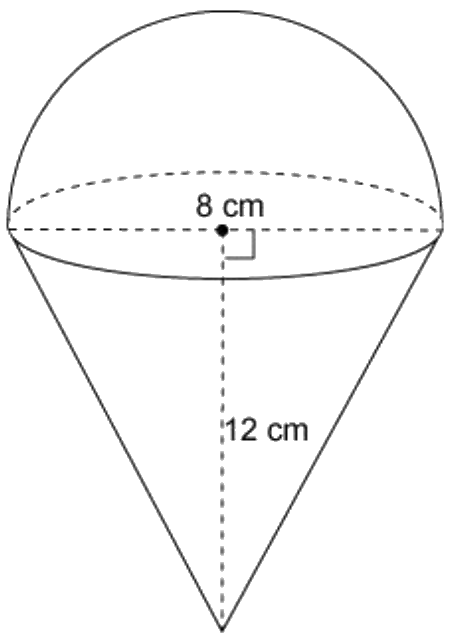
\includegraphics[width=0.17\textwidth]{Figuras/fig53.png}
\vspace{-15pt}
\end{wrapfigure}

Observa el helado de la figura.

\textbf{a)} Halla el volumen de la figura.

\textbf{b)} Si el volumen del helado (cono más hemisferio) fuera de 600 cm$^3$, y el radio del círculo no cambiara, ¿cuál tendría que ser la altura del cono?

\vspace{6mm}

%\newpage

% ========== ACTIVIDAD 2 ==========
\section*{ACTIVIDAD 2: VOLUMEN Y ÁREA SUPERFICIAL DE SÓLIDOS}

\textit{Continuemos analizando sólidos y exploremos más a fondo las áreas superficiales, usando sólidos y figuras planas básicas como ayuda para encontrarlas.}

\subsection*{A) Activando saberes previos}

\begin{tcolorbox}[colback=fondoazul, colframe=azuloscuro, title=\textbf{RECUERDA QUE...}, breakable]
\begin{itemize}[nosep]
    \item El área superficial de un prisma o de un cilindro circular es igual a su área lateral más dos veces el área de cada base.
\end{itemize}

\begin{center}
\small
\begin{tabular}{|
		>{\centering\arraybackslash}m{4.5cm}|
		>{\centering\arraybackslash}m{4.5cm}|
		>{\centering\arraybackslash}m{2.5cm}|}
\hline
\textbf{Sólido} & \textbf{Área Superficial} & \textbf{Figura} \\
\hline
Cubo de lado $L$ & $A = 4L^2 + 2L^2 = 6L^2$ & 
\includegraphics[width=1.5cm]{Figuras/fig44.png} \\
\hline
Prisma con base triangular equilátera de lado $X$ y altura $H$ & $A = 3XH + 2\frac{\sqrt{3}}{4}X^2$ & 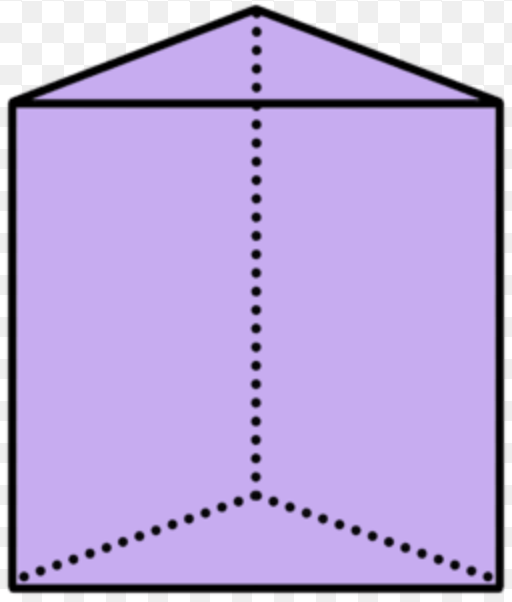
\includegraphics[width=1.2cm]{Figuras/fig82b.png} \\
\hline
Cilindro de radio $R$ y altura $H$ & $A = 2\pi RH + 2\pi R^2$ & 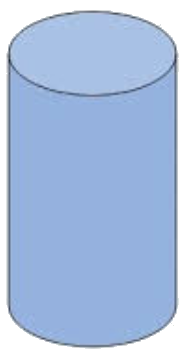
\includegraphics[width=.8cm]{Figuras/fig5.png} \\
\hline
Tetraedro regular de lado $X$ & $A = 4\frac{\sqrt{3}}{4}X^2 = \sqrt{3}X^2$ & 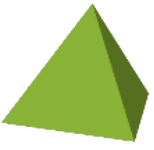
\includegraphics[width=1.5cm]{Figuras/fig43.png} \\
\hline
\end{tabular}
\end{center}
\end{tcolorbox}

\begin{tcolorbox}[colback=fondoverde, colframe=verdeclaro, title=\textbf{PRACTICA}, breakable]
\textbf{i)} Completa esta tabla, marcando con \checkmark\ o X según el sólido tenga o no la propiedad dada.

\begin{center}
\small
\begin{tabular}{|
		>{\centering\arraybackslash}m{2.5cm}|
		>{\centering\arraybackslash}m{2cm}|
		>{\centering\arraybackslash}m{1.5cm}|
		>{\centering\arraybackslash}m{2cm}|
		>{\centering\arraybackslash}m{1.5cm}|
		>{\centering\arraybackslash}m{2cm}|}
\hline
\textbf{Sólido} & \textbf{Poliedro regular} & \textbf{Prisma} & \textbf{Pirámide} & \textbf{1 cara} & \textbf{Cilindro circular} \\
\hline
Elipsoide \newline 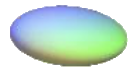
\includegraphics[width=1.8cm]{Figuras/fig54.png} & & & & & \\
\hline
Dodecaedro \newline \includegraphics[width=1.8cm]{Figuras/fig55.png} & & & & & \\
\hline
Ortoedro \newline \includegraphics[width=1.8cm]{Figuras/fig56.png} & & & & & \\
\hline
\end{tabular}
\end{center}

\textbf{ii)} Halla el área de un cilindro circular cuya base tiene un área de $16\pi$ unidades cuadradas, y cuyo radio de la base, $R$, es la mitad de la altura, $H$.

\textbf{iii)} Considera un tetraedro regular en donde cada lado de cada triángulo equilátero mide 2 unidades.

Basado en esto, encuentra el área de superficie del tetraedro.
\end{tcolorbox}

\vspace{4mm}

%\newpage

\subsection*{B) Conceptos}

\subsubsection*{Exploremos: Pintando o recubriendo los prototipos}

\begin{tcolorbox}[colback=fondoverde, colframe=verdeclaro]
Antes de comenzar discute en clase: ¿cuando miras las caras 2D de los objetos de tu vida cotidiana, ¿cuáles son planas? Y las que no lo son, ¿podrían aplanarse? Explica.
\end{tcolorbox}

La misma diseñadora de la Actividad 1 tiene ya listos sus prototipos, ya ha encontrado volúmenes y contado vértices, aristas y caras de los módulos que son poliedros. Ahora es tiempo de pintar o recubrir la superficie de cada prototipo (sus caras planas y redondas) y para ello debemos estimar su \textbf{ÁREA SUPERFICIAL} de ellos, medidos en cm$^2$ o m$^2$, según sea conveniente. Exploremos algunos de ellos.

Recordemos los sólidos básicos que usará la diseñadora, y el área (superficial) de cada uno de ellos:

\begin{center}
\begin{tabular}{|
	>{\centering\arraybackslash}m{4cm}|
	>{\centering\arraybackslash}m{4cm}|
	>{\centering\arraybackslash}m{4cm}|}
\hline
\textbf{Cilíndricos} & \textbf{Puntiagudos} & \textbf{Esféricos} \\
\hline
\textbf{Prisma}

\includegraphics[width=3cm]{Figuras/fig60.png}

Área: se suman las áreas de las 2 bases más las áreas de los lados, que son polígonos. &
\textbf{Pirámide}

\includegraphics[width=4cm]{Figuras/fig62.png}

Área: Se suma el área de la base más $n$ veces el área de cada cara lateral (que es un triángulo), donde $n$ es el número de caras. &
\textbf{Esfera y hemisferio} (``Pelotas'')

\includegraphics[width=3cm]{Figuras/fig64.png}

Área de una esfera de radio $R$:
$$4\pi R^2$$ \\
\hline
\textbf{Cilindro circular}

\includegraphics[width=3cm]{Figuras/fig61.png}

Área del cilindro de radio $R$ y altura $H$:
\begin{itemize}[nosep]
    \item Cada base: $\pi R^2$
    \item Lado: $2\pi RH$
\end{itemize}

Área total = $2\pi R^2 + 2\pi RH$ &
\textbf{Cono}

\includegraphics[width=1.9cm]{Figuras/fig63.png}

Área del cono de radio $R$ y altura $H$:
\begin{itemize}[nosep]
    \item Base: $\pi R^2$
    \item Lado: $\pi R\sqrt{H^2 + R^2}$
\end{itemize}

Área total: $\pi R^2 + \pi R\sqrt{H^2 + R^2}$ & \\
\hline
\end{tabular}
\end{center}

\vspace{4mm}

%\newpage

\textbf{i) El sofá:}

\begin{wrapfigure}{r}{0.35\textwidth}
\centering
\includegraphics[width=0.33\textwidth]{Figuras/fig67.png}
\end{wrapfigure}

Supongamos que los dos módulos son ortoedros iguales, cada uno de dimensiones $X$, $Y$ y $Z$ m, en donde $X < Y < Z$.

El área superficial del prisma A1 es la suma de áreas de sus 6 lados:
$$A1 = 2XY + 2XZ + 2YZ.$$

\begin{wrapfigure}{l}{0.35\textwidth}
\centering
\includegraphics[width=0.33\textwidth]{Figuras/fig66.png}
\end{wrapfigure}

¿Qué sucede al pegarlos? Cuando pegamos los módulos, los estamos pegando en un rectángulo de dimensiones $X$ por $Z$. Entonces ese rectángulo no se va a recubrir en ninguno de los dos módulos.

Concluimos que el área superficial del sofá es:
$$A = 2XY + 2XZ + 2YZ - 2XZ = 2Y(X + Z) \text{ m}^2.$$

\subsubsection*{Responde:}

\textbf{a)} Si a la diseñadora no le interesara recubrir la parte de abajo del sofá, ¿cuál sería el área superficial? ¡Escribe la fórmula!

\textbf{b)} Inventa valores plausibles para las dimensiones del sofá y halla su área superficial.

\vspace{4mm}

%\newpage

\textbf{ii) La cabaña:}

\begin{wrapfigure}{r}{0.25\textwidth}
\centering
\includegraphics[width=0.25\textwidth]{Figuras/fig68.png}
\end{wrapfigure}

Las dos piezas en que hemos separado la choza son un prisma rectangular y una pirámide de base rectangular (igual a la cara superior del prisma).

¿Cuántas longitudes hay en esta situación?

Una forma de verlo es que hay 4 longitudes):
\begin{itemize}[nosep]
    \item $X$ y $Y$: las dimensiones del rectángulo común
    \item $Z$: la altura del prisma
    \item $W$: la altura de la pirámide.
\end{itemize}

($Z + W$ es la distancia del suelo a la punta de la cabaña).

El prisma nos aporta sus 4 caras laterales en cuanto a área:
$$2XZ + 2YZ = 2Z(X + Y)$$

\begin{wrapfigure}{l}{0.35\textwidth}
\centering
\includegraphics[width=0.33\textwidth]{Figuras/fig69.png}
\end{wrapfigure}

La pirámide aporta sus 4 caras triangulares. 2 de ellas son iguales y con $X$ como base; las otras 2 son iguales, y con $Y$ como base.

\textbf{Cara triangular de base $Y$:}

Podemos usar el Teorema de Pitágoras para hallar la altura $H$: Sabemos que $W^2 + (X/2)^2 = H^2$.

Entonces $H = \sqrt{W^2 + X^2/4}$. Entonces el área del triángulo de base $Y$ es: $\frac{1}{2}Y\sqrt{W^2 + X^2/4}$.

\textbf{Cara triangular de base $X$:}

De forma muy similar, el área del triángulo de base $X$ es: $\frac{1}{2}X\sqrt{W^2 + Y^2/4}$.

Así, el área por recubrir para la pirámide (4 triángulos) es: $Y\sqrt{W^2 + X^2/4} + X\sqrt{W^2 + X^2/4}$.

Sumando, el área de recubrimiento de la cabaña es:
$$A = 2Z(X + Y) + Y\sqrt{W^2 + X^2/4} + X\sqrt{W^2 + X^2/4}.$$

\vspace{4mm}

%\newpage

\begin{tcolorbox}[colback=fondorosa, colframe=rojoclaro, title=\textbf{Mini-explicación: Área superficial: ¿cuánto se necesita para cubrir la superficie de un sólido?}, breakable]
\textbf{ÁREA SUPERFICIAL}

El área superficial de un sólido es una medida de área que nos dice cuánto se necesita para recubrir la superficie del mismo.

Según la situación, a veces NO necesitamos cubrir todo el sólido, sino algunas de sus caras (ya sean planas o no planas).

\begin{wrapfigure}{r}{0.25\textwidth}
\centering
\vspace{-10pt}
\includegraphics[height=2.5cm]{Figuras/fig70.png}
\vspace{-10pt}
\end{wrapfigure}

Si el sólido es una pirámide cuadrada, entonces tiene 5 caras: una cuadrada y 4 triangulares. Como en la página anterior (caso general de pirámide rectangular), el área superficial es igual a

ÁREA DE CUADRADO + 4 VECES EL ÁREA DE CADA CARA TRIANGULAR:
$$A = a^2 + 2a\sqrt{h^2 + a^2/4}.$$

($a$ = lado del cuadrado; $h$ = altura de la pirámide)

\begin{wrapfigure}{l}{0.25\textwidth}
\centering
\vspace{-10pt}
\includegraphics[height=2.5cm]{Figuras/fig71.png}
\vspace{-10pt}
\end{wrapfigure}

Si el sólido es una pirámide cuya base es un polígono regular de $n$ lados (por ejemplo, un hexágono regular), entonces su área es igual al área de la base + $n$ veces el área de cada triángulo lateral.

El área del triángulo lateral se calcula usando el teorema de Pitágoras, como en el caso anterior. La expresión que obtienes debe depender del lado de la base y de la altura de la pirámide.

\begin{wrapfigure}{r}{0.48\textwidth}
\centering
\vspace{-10pt}
\includegraphics[height=2.5cm]{Figuras/fig72.png}
\vspace{-10pt}
\end{wrapfigure}

Si el sólido es un cono de radio $r$ y altura $h$, entonces podemos hallar su generatriz $l$ usando Pitágoras: $l = \sqrt{h^2 + r^2}$.

Desenrrollando el cono (aplanándolo), nos quedan dos figuras: el círculo base, y un sector circular con radio $l$ y arco $2\pi r$.

Recordando que el área de un sector circular es la mitad del producto radio $\times$ arco, entonces el área superficial del cono es:
$$A = \pi r^2 + \pi rl = \pi r(r + \sqrt{h^2 + r^2}).$$

\begin{wrapfigure}{l}{0.25\textwidth}
\centering
\vspace{-40pt}
\includegraphics[height=2.5cm]{Figuras/fig73.png}
\vspace{-10pt}
\end{wrapfigure}

En el caso de una esfera de radio $r$, el área superficial es $A = 4\pi r^2$.

Un hemisferio de radio $r$ tiene dos caras: una es media esfera y la otra un círculo de radio $r$. Así, su área es $A = 2\pi r^2 + \pi r^2 = 3\pi r^2$.
\end{tcolorbox}

\vspace{4mm}

%\newpage

\subsubsection*{Ejemplo: El área superficial de un cono truncado}

\begin{wrapfigure}{r}{0.3\textwidth}
\centering
\includegraphics[width=0.28\textwidth]{Figuras/fig22.png}
\end{wrapfigure}

Supongamos que la caperuza de la lámpara es la parte inferior de un cono de base circular de radio 21 cm y altura 90 cm.

El cono superior es lo que quedaría si le quitamos la caperuza al cono entero. Tiene altura 60 cm.

Supongamos además que la altura de la caperuza es 30 cm.

¿Cómo podemos hallar el área de la caperuza?

\begin{wrapfigure}{l}{0.25\textwidth}
\centering
\includegraphics[width=0.25\textwidth]{Figuras/fig74.png}
\end{wrapfigure}

Primero podemos hallar el área del cono (sin su base), que es igual a $\pi r\sqrt{h^2 + r^2}$, es decir a $21\pi\sqrt{8100 + 441} \approx 6097$ cm$^2$.

Usando triángulos semejantes y proporcionalidad, la razón 60 : 90 entre la altura de la pirámide superior y la altura de todo el cono, debe ser igual a la razón de los radios de las bases de los conos. Así, si llamamos $P$ al radio de la base del cono superior, entonces 60 : 90 es la misma proporción que $P$ : 21. En fracciones: $\frac{60}{90} = \frac{P}{21}$, entonces $P = 14$ cm.

Esto nos ayuda entonces a encontrar el área del cono superior (sin su base), que es igual a $\pi p\sqrt{60^2 + p^2}$, es decir a $14\pi\sqrt{3600 + 196} \approx 2710$ cm$^2$.

Jairo, un amigo de la diseñadora y quien va a ayudarle con el recubrimiento, le dice que si la caperuza tiene la tercera parte de la altura del cono, entonces por qué su área no es simplemente la tercera parte de 6097? (es decir, 2032,3)?

La diseñadora le responde: ``Jairo, si estuviéramos trabajando con un cilindro, tu lógica sería correcta. Pero mira la forma de un cono. Cerca de la base tiene más volumen que arriba, y también tiene más área superficial. Así que no podemos usar la regla de 3 que me propones.''. Jairo comprende y le da la razón.

\vspace{4mm}

%\newpage

\subsubsection*{Paso 2: Completa este ejemplo: Partiendo una esfera en 8 pedazos iguales}

Queremos hacer un rompecabezas geométrico que consiste en dividir una esfera sólida de radio $R = 64$ cm en 8 pedazos iguales. Cada pedazo lo vamos a cubrir con muchas ``escamas'' cuadradas de aproximadamente 0,4 cm$^2$ cada una y queremos averiguar cuántas necesitamos para cada pedazo.

Completa el siguiente diagrama, en donde cada vez partimos la figura en 2 partes iguales:

\begin{center}
\small
\begin{tabular}{|
		>{\centering\arraybackslash}m{3cm}|
		>{\centering\arraybackslash}m{3cm}|
		>{\centering\arraybackslash}m{3cm}|
		>{\centering\arraybackslash}m{3.5cm}|}
\hline
\textbf{Esfera (E)} & \textbf{Hemisferio (medio E)} & \textbf{Cuarto de esfera} & \textbf{Octavo de esfera} \\
\hline
\begin{tikzpicture}[scale=0.99]
\shade[ball color=blue!30!brown] (0,0) circle (1);
\draw[thick] (0,0) circle (1);
\end{tikzpicture}
&
\begin{tikzpicture}[scale=0.99]
\draw[thick, ball color=blue!30!brown] (-1,0) arc (180:0:1) -- cycle;
\draw[thick, ball color=blue!55] (0,0) ellipse (1 and 0.25);
\draw[thick, dashed] (-1,0) arc (180:360:1 and 0.25);
\end{tikzpicture}
&
\begin{tikzpicture}[scale=0.99]
\draw[thick, ball color=blue!55] (0,0) -- (1,0) arc (0:-90:1) -- cycle;
%\draw[thick, fill=blue!20] (0,0) arc (180:90:1 and 0.25) -- (0,0.25) -- cycle;
\draw[thick] (1,0) arc (0:-90:1);
\draw[thick, ball color=blue!30!brown] (0,0) arc (180:0:.5 and 0.25);
\end{tikzpicture}
&
\begin{tikzpicture}[scale=0.99]
	\draw[thick, ball color=blue!55] (0,0) -- (1,0) arc (0:-90:1) -- cycle;
	%\draw[thick, fill=blue!20] (0,0) arc (180:90:1 and 0.25) -- (0,0.25) -- cycle;
	\draw[thick] (1,0) arc (0:-90:1);
	\draw[thick, ball color=blue!30!brown] (0,0) arc (180:0:.5 and 0.125);
\end{tikzpicture}
\\
\hline
\end{tabular}
\end{center}

\textbf{a)} Completa la siguiente tabla de los volúmenes.

\begin{center}
\begin{tabular}{|p{3.5cm}|p{4.5cm}|p{4.5cm}|}
\hline
\textbf{Sólido} & \textbf{Descripción alterna} & \textbf{Volumen} \\
\hline
Esfera & Dos hemisferios juntos & $\frac{4}{3}\pi R^3 = \frac{4}{3}\pi \cdot 64^3$ cm$^3$ \\
\hline
Media esfera & ? & ? \\
\hline
Cuarto de esfera & ? & ? \\
\hline
Octavo de esfera & ? & ? \\
\hline
\end{tabular}
\end{center}

\textbf{b)} Hallemos el área superficial de medio hemisferio.

Este tiene 2 caras planas, cada una es medio círculo. Su cara redonda tiene la cuarta parte del área superficial de la esfera (el cual es $4\pi R^2$). Identifica estas caras en tu dibujo y halla el área superficial.

\textbf{c)} Completa la siguiente tabla de los áreas superficiales. Recuerda que salvo la esfera, los sólidos tienen más de una cara.

\begin{center}
\begin{tabular}{|p{3.5cm}|p{4.5cm}|p{4.5cm}|}
\hline
\textbf{Sólido} & \textbf{Descripción alterna} & \textbf{Área de superficie} \\
\hline
Esfera & Dos hemisferios juntos & $4\pi R^2 = 4\pi \cdot 64^2$ cm$^2$ \\
\hline
Media esfera & ? & $2\pi R^2 + \pi R^2 = ?$ \\
\hline
Cuarto de esfera & ? & ? \\
\hline
Octavo de esfera & ? & ? \\
\hline
\end{tabular}
\end{center}

\vspace{4mm}

%\newpage

\subsubsection*{Paso 3: 1-2-4: Tu turno (individual, en parejas y en grupos de 4)}

\begin{wrapfigure}{r}{0.35\textwidth}
\centering
\includegraphics[width=0.33\textwidth]{Figuras/fig77.png}
\end{wrapfigure}

Tienes una pirámide de base cuadrada de lado $a = 10$, y altura $h = 12$.

\textbf{a)} Encuentra el área superficial de la pirámide, sin incluir su base.

\textbf{b)} Corta la pirámide por la mitad, paralelo a la base, de forma que te queden 2 piezas: una pirámide truncada de altura $h/2$, y una pirámide pequeña de altura $h/2$ también. Haz un dibujo. ¿Cuáles son las dimensiones del cuadrado base de la pirámide pequeña?

\textbf{c)} Encuentra el área superficial de la pirámide truncada (no incluyas ni su tapa ni su base.

Júntate con otro estudiante e intercambien sus procesos de solución, trabajando en equipo. Anoten sus dudas comunes.

Júntense con otra pareja y compartan sus soluciones. Encuentren errores o dibujos que puedan mejorar.

Finalmente, busquen a su profesor para dialogar y compartir sus estrategias y respuestas, aclarando los conceptos.

\begin{tcolorbox}[colback=fondorosa, colframe=rojoclaro, title=\textbf{PROYECTO GRUPAL - APLIQUEMOS LO APRENDIDO}, breakable]
Formen grupos de 4 estudiantes. Vamos a trabajar en un proyecto para aplicar lo que aprendimos.

\textbf{Instrucciones:}

\begin{enumerate}[nosep]
    \item Elijan un sólido que combine creativamente una esfera, un cono y una pirámide, o partes de ellas. No vale sólo pegar esta 3 separadamente (porque entonces uno simplemente sumaría). Generen formas novedosas. Inventen un nombre para el sólido.

    \item Entre todos, hagan una lluvia de ideas acerca de cómo usar lo aprendido para aproximar o hallar el área de superficie del sólido.

    \item Apliquen sus ideas para encontrar la respuesta, que será una expresión con variables. No importa si hacen aproximaciones, exploren nuevas formas de pensar.

    \item Elaboren una cartelera física o digital para exponer sus ideas en su clase. Incluyan tablas, gráficas y otros recursos visuales.
\end{enumerate}
\end{tcolorbox}

\vspace{4mm}

%\newpage

\subsection*{C) Resuelve y practica}

\begin{multicols}{2}

\textbf{1)} Dibuja los siguientes patrones en cartulina. Después, arma los sólidos correspondientes, tomando las medidas necesarias y calcula el área superficial total aproximada de cada uno.

\textbf{a)} Pentágono regular

\begin{center}
\includegraphics[width=0.25\textwidth]{Figuras/fig79.png}
\end{center}

\vspace{2mm}

\textbf{b)} Cubo

\begin{center}
\includegraphics[width=0.25\textwidth]{Figuras/fig80.png}
\end{center}

\vspace{2mm}

\textbf{c)} Pirámide triangular

\begin{center}
\includegraphics[width=0.25\textwidth]{Figuras/fig81.png}
\end{center}

\vspace{2mm}

\textbf{d)} Cono con sector circular

\begin{center}
\includegraphics[width=0.25\textwidth]{Figuras/fig82.png}
\end{center}

\vspace{2mm}

\textbf{2)} En el conjunto residencial ``Los Áticos'' están construyendo un tanque, en forma de ortoedro, para almacenamiento de agua, cuyas dimensiones son: 5 m de largo, 4 m de ancho y 3 m de profundidad. Ayuda al ingeniero de la obra a resolver los siguientes interrogantes:

\textbf{a)} ¿Cuántos metros cuadrados de revestimiento impermeabilizante debe comprar para cubrir las paredes, el piso y el techo del tanque?

\textbf{b)} ¿Cuántos metros cúbicos de agua puede almacenar el tanque? Si cada medida creciera en 1m, ¿en cuánto aumentaría el volumen del tanque?

\textbf{3)} Da 4 ejemplos de conos distintos que tengan un área de superficie cercana a 12 unidades cuadradas. Dibuja los 4 conos y ordénalos ascendentemente según la fracción ``altura / radio de la base''.

\textbf{4)} Haz varios dibujos posibles para el siguiente problema, y después resuélvelo: ``El perímetro de la base de un prisma triangular recto mide 15 cm. Halla el área lateral del prisma si la altura del prisma es 12 cm.''

\textbf{5)} Calcula el área de cada cara, el área superficial total y el volumen de un prisma de base cuadrada con lado de la base 8 cm y la altura 12 cm. Aproxima cada respuesta a un entero.

\textbf{6)} Calcula el área superficial y el volumen de un cubo de 12 cm de arista.

\textbf{7)} Halla el volumen de un globo esférico de 80 cm de radio.

\textbf{8)} Halla el área de un cono de 5 m de radio y 8 m de altura.

\textbf{9)} Calcula la superficie de cuero que se necesita para hacer un balón de fútbol de 9 cm de radio.

\textbf{10)} Halla el área superficial de una esfera de $3X$ m de radio.

\textbf{11)} Calcula el volumen de un cono si el radio de la base es de 25 cm y la altura es de 400 cm. Expresa tu respuesta en m$^3$.

\textbf{12)} Calcula la diferencia entre los volúmenes de dos esferas concéntricas (es decir, con el mismo centro) de 15 cm de radio una y de 10 cm la otra.

\end{multicols}

\vspace{4mm}

%\newpage

\subsection*{D) Resumen}

\begin{center}
\textbf{SÓLIDOS}

$\downarrow$

Reconocer sus caras (planas y curvas)

$\downarrow$

Usarlas para encontrar

$\downarrow$

\textbf{ÁREA DE SUPERFICIE}
\end{center}

\begin{tcolorbox}[colback=fondoazul, colframe=azuloscuro, title=\textbf{ÁREAS DE SUPERFICIE}, breakable]
\begin{center}
\begin{tabular}{|
		>{\centering\arraybackslash}m{3.5cm}|
		>{\centering\arraybackslash}m{3.5cm}|
		>{\centering\arraybackslash}m{3.5cm}|}
\hline
\textbf{Cilíndricos} & \textbf{Puntiagudos} & \textbf{Esféricos} \\
\hline
\textbf{Prisma}

Área: se suman las áreas de las 2 bases más las áreas de los lados, que son polígonos. &
\textbf{Pirámide}

Área: Se suma el área de la base más $n$ veces el área de cada cara lateral (que es un triángulo), donde $n$ es el número de caras. &
\textbf{Esfera y hemisferio} (``Pelotas'')

Área de una esfera de radio $R$:
$$4\pi R^2$$ \\
\hline
\textbf{Cilindro circular}

Área del cilindro de radio $R$ y altura $H$:
\begin{itemize}[nosep]
    \item Cada base: $\pi R^2$
    \item Lado: $2\pi RH$
\end{itemize}

Área total = $2\pi R^2 + 2\pi RH$ &
\textbf{Cono}

Área del cono de radio $R$ y altura $H$:
\begin{itemize}[nosep]
    \item Base: $\pi R^2$
    \item Lado: $\pi R\sqrt{H^2 + R^2}$
\end{itemize}

Área total: $\pi R^2 + \pi R\sqrt{H^2 + R^2}$ & \\
\hline
\end{tabular}
\end{center}
\end{tcolorbox}

\begin{tcolorbox}[colback=fondoverde, colframe=verdeclaro, title=\textbf{Ten en cuenta que:}, breakable]
\begin{itemize}[nosep]
    \item Para hallar el área superficial de una pirámide es útil el Teorema de Pitágoras, que permite hallar la altura de cada cara triangular.
    \item Es importante reconocer en cada problema de conos y cilindros si las ``tapas'' o ``base'' se deben incluir en el cálculo del área supeficial.
    \begin{itemize}[nosep]
        \item Por ejemplo, si se quiere pintar un cono de helado, entonces NO se necesita pintar su cara circular. Pero en cambio si se tiene una caneca abierta, entonces sí se debe pintar su base circular.
    \end{itemize}
    \item Todas las fórmulas de área superficial son suma de términos en donde se tiene un número fijo y el producto de dos variables (a veces iguales). Esto nos ayuda fácilmente a detectar errores en el álgebra.
\end{itemize}
\end{tcolorbox}

\vspace{4mm}

%\newpage

\subsection*{E) Valoración}

\textbf{i) Califica tu comprensión por tema en tu cuaderno}

\begin{center}
\small
\begin{tabular}{|
		>{\centering\arraybackslash}m{5.5cm}|
		>{\centering\arraybackslash}m{2.5cm}|
		>{\centering\arraybackslash}m{2.5cm}|
		>{\centering\arraybackslash}m{2.5cm}|}
\hline
\textbf{Tema} & \textbf{$\bullet\circ\circ$ No entiendo (TODAVÍA)} & \textbf{$\bullet\bullet\circ$ Voy bien} & \textbf{$\bullet\bullet\bullet$ Comprendí bien} \\
\hline
Identifico las caras de un sólido y su naturaleza (planas o no planas) & & & \\
\hline
Razono para hallar el área superficial de una pirámide & & & \\
\hline
Razono para hallar el área superficial de de un cono & & & \\
\hline
Razono para hallar el área superficial de una esfera & & & \\
\hline
\end{tabular}
\end{center}

\textbf{ii) Preguntas de comprensión}

\textbf{1)} Si cada lado de un cubo se multiplica por 4, entonces el área superficial del cubo...

[ ] se multiplica por 8.

[ ] se multiplica por 16.

\textbf{2)} Si cada área de cara de un cubo se multiplica por 3, entonces el área superficial del cubo...

[ ] se multiplica por 3.

[ ] se multiplica por 9.

\textbf{3)} Si la altura de un cono y el diámetro de su base se multiplican cada uno por 10, entonces el área superficial del cono...

[ ] se multiplica por 10.

[ ] se multiplica por 100.

\textbf{4)} Si el volumen de una esfera se reduce a 1/64, entonces el área superficial...

[ ] se reduce a 1/16.

[ ] se reduce a 1/32.

(Verifica las respuestas con tu profesor)

\vspace{4mm}

%\newpage

\textbf{iii) Resuelvo un problema}

Tenemos una esfera de 10 cm de diámetro.

\textbf{a)} Calcula el área superficial de la esfera.

\textbf{b)} Si el diámetro de la esfera aumenta en un 50\%, ¿en qué porcentaje aumenta su área superficial? Muestra tus cálculos y razonamiento.

\vfill

\begin{center}
\textbf{FIN DE LA GUÍA 85}
\end{center}

\end{document}
